\documentclass[12pt]{report}

%This is the main thesis file. Even though the chapter contents are saved in other files, you must always TeXify %from the main file.

\usepackage{amsmath,amsthm,amssymb}
\usepackage{setspace}
\usepackage[mathscr]{eucal}
\usepackage{wrapfig}
\usepackage{graphicx}
\usepackage{psfrag}
\usepackage{ifthen}
\usepackage{array}
\usepackage{longtable}
\usepackage{fancyvrb}
\usepackage{fancyhdr}
\usepackage{color}
\usepackage{sectsty}
\usepackage[calcwidth]{titlesec}
\usepackage{tocloft}
\usepackage{float}
\usepackage{indentfirst,microtype}
\usepackage{algorithm}
\usepackage{algpseudocode}
\usepackage{subfigure}
\usepackage{comment}
\usepackage{tabularx}
\usepackage{multirow}
\usepackage{pdfpages}
% \usepackage{lineomath}
\usepackage[labelfont=bf]{caption} %For bold label for figures and tables (for indented captions, use the "hang" option.

\AtBeginDocument{\setlength\abovedisplayskip{3pt}}
\AtBeginDocument{\setlength\belowdisplayskip{3pt}}

\renewcommand{\cfttoctitlefont}{\large\bfseries}
\renewcommand{\cftloftitlefont}{\large\bfseries}
\renewcommand{\cftlottitlefont}{\large\bfseries}

%\setlength{\cftbeforetoctitleskip}{42pt}
%\setlength{\cftaftertoctitleskip}{12pt}
\setlength{\cftbeforeloftitleskip}{42pt}
\setlength{\cftafterloftitleskip}{12pt}
\setlength{\cftbeforepartskip}{0pt}
\setlength{\cftbeforechapskip}{0pt}
\setlength{\cftbeforesecskip}{0pt}
\setlength{\cftbeforesubsecskip}{0pt}
\newcommand*{\noaddvspace}{\renewcommand*{\addvspace}[1]{}}
\addtocontents{lof}{\protect\noaddvspace}
\setlength{\parskip}{0in}%{2ex plus0.5ex minus0.2ex}
\setlength{\parindent}{0.5in}

%This uses sectsty package to change the style of the headings.
%\allsectionsfont{\sffamily\underline}
%\allsectionsfont{\large\centering\underline}
%\sectionfont{\normalfont\sffamily\large\underline\bfseries}
%\subsectionfont{\normalsize\underline}

%This will underline section and subsection headings
%\titleformat{\section}{\large\centering\bfseries}{\thesection}{1em}{}%{\uline}
%\titleformat{\subsection}{\normalsize\bfseries}{\thesubsection}{1em}{\uline}

\newlength{\SpaceBeforeChapter}
\setlength{\SpaceBeforeChapter}{0.55in}



\setlength{\textwidth}{6in}% 8.5 - 1in - 1.5in = 6in
\setlength{\textheight}{9in}% 11 - 1in - 1in = 9in
% The height of the header
\setlength{\headheight}{0.202in}
% the space between the header and the start of the document is 0.5 - .202, because we want 1in margins
\setlength{\headsep}{0.298in}
% We want the page number to display 0.5 inches from the bottom of the text
\setlength{\footskip}{0.5in }
% This will make the right margin 1in + 0.5
\setlength{\oddsidemargin}{0.5in}
\setlength{\evensidemargin}{0.5in}
% No horizontal offset is needed
\setlength{\hoffset}{0pt}
% We want the header to begin showing at 1.0in + \voffset ~ which is 0.5 for the page number
\setlength{\voffset}{-0.5in}
\setlength{\topmargin}{0pt}

% To create triple spacing, we use single spacing, then add 3ex to create triple spacing ~ there may be a more correct way to do this
\titleformat{\chapter}[display]{\singlespacing\centering\large\bfseries}{\MakeUppercase{\chaptertitlename}~\thechapter}{4ex}{\setlength{\parskip}{0pt}\large\uppercase}[\setlength{\parskip}{0pt}]%{0pt}]
\titlespacing{\chapter}{0pt}{\SpaceBeforeChapter}{2.5ex}

% Section headers should have a triple space before them (3ex), and a double space after (2ex)
\titleformat{\section}[block]{\singlespacing\centering\normalsize\bfseries}{\thetitle}{1ex}{\normalsize}
\titlespacing{\section}{0pt}{3ex}{0ex}

% Subsection headers should have a double space before them (2ex), and a double space after (2ex)
% And they should not be centered
\titleformat{\subsection}{\singlespacing\normalsize\bfseries}{\thetitle}{1ex}{}
\titlespacing{\subsection}{0pt}{3pt}{0ex}
%\titlespacing{\subsection}{0pt}{2ex}{0ex} %original LMK, double space better expressed with 3pt

%spacing for subsubsections
\titlespacing{\subsubsection}{0pt}{3pt}{0ex}

\newcounter{currpart}


\renewcommand{\cftpartfont}{\normalfont}
\renewcommand{\cftpartpagefont}{\normalfont}
\renewcommand{\cftchapfont}{\normalfont}
\renewcommand{\cftchappagefont}{\normalfont}
\renewcommand{\cftchappresnum}{CHAPTER }
\renewcommand{\cftpartpresnum}{PART }
\renewcommand{\cftfigpresnum}{Figure }
\renewcommand{\cftfigaftersnum}{:}
\renewcommand{\cfttabaftersnum}{:}
\renewcommand{\cftchapnumwidth}{7em}
\renewcommand{\cftfignumwidth}{5.5em}
\renewcommand{\cfttabnumwidth}{5.5em}

%\renewcommand{\cftXdotsep}{0}

\renewcommand{\cftpartleader}{\cftdotfill{\cftsecdotsep}}
\renewcommand{\cftchapleader}{\cftdotfill{\cftsecdotsep}}
\renewcommand{\cftdotsep}{0}
\cftsetpnumwidth{1.3em} %1 in LMK's thesis, increased to take care of wide roman numerals
\setlength{\cftchapindent}{0pt}
\setlength{\cftfigindent}{0pt}
\setlength{\cfttabindent}{0pt}
\addtocontents{lof}{\protect\noaddvspace}
\addtocontents{lot}{\protect\noaddvspace}

%\setlength{\itemsep}{0ex}
%\setlength{\topsep}{0ex}
%\setlength{\partopsep}{0ex}

  \let\oldthebibliography=\thebibliography
  \let\endoldthebibliography=\endthebibliography
  \renewenvironment{thebibliography}[1]{%
    \begin{oldthebibliography}{#1}%
      \setlength{\parskip}{0pt}%
      \setlength{\itemsep}{0pt}%
  }%
  {%
    \end{oldthebibliography}%
  }


  \let\olditemize=\itemize
  \let\endolditemize=\enditemize
  \renewenvironment{itemize}{%
\vspace{-.15in} %hard codes the vertical space before the environment
    \begin{olditemize}%
\setlength{\parsep}{0ex}
\setlength{\topsep}{0ex}
\setlength{\partopsep}{0ex}
      \setlength{\parskip}{0pt}%
      \setlength{\itemsep}{0pt}%
  }%
  {%
    \end{olditemize}%
  }

  \let\oldenumerate=\enumerate
  \let\endoldenumerate=\endenumerate
  \renewenvironment{enumerate}{%
\vspace{-.15in} %hard codes the vertical space before the environment
    \begin{oldenumerate}%
\setlength{\parsep}{0ex}
\setlength{\topsep}{0ex}
\setlength{\partopsep}{0ex}
      \setlength{\parskip}{0pt}%
      \setlength{\itemsep}{0pt}%
  }%
  {%
    \end{oldenumerate}%
  }



\renewcommand{\baselinestretch}{2.0}
%Main file to compile the thesis.
%DO NOT CHANGE THIS FILE, EXCEPT FOR THE INCLUDE COMMANDS

%\flushbottom
\allowdisplaybreaks

    % THIS WILL FORCE EQUATION NUMBERS TO START OVER WITH EACH
    % NEW CHAPTER
    \numberwithin{equation}{chapter}
    \renewcommand{\theequation}
        {\arabic{chapter}.\arabic{equation}}
    \renewcommand{\thefigure}
        {\arabic{chapter}.\arabic{figure}}
    \renewcommand{\thetable}
        {\arabic{chapter}.\arabic{table}}

    % using fancyhdr ............................................
    \pagestyle{fancy}
    \renewcommand{\chaptermark}[1]
    {\markboth{\textit{\chaptername\ \thechapter.\ #1}}{}}
    % the header
    \lhead{}%{\textit{Your Name}}
    \chead{}%{\leftmark}
    \rhead{\thepage}
    % the footer
    %\lfoot{}
    \cfoot{}
    \rfoot{}
    \renewcommand{\headrulewidth}{0pt}
    \renewcommand{\footrulewidth}{0pt}

    \title{Your Title}
    \author{Your Name}
    \date{Month Year}

\newcommand{\ds}{\displaystyle}
\newcommand{\p}{\partial}
\newcommand{\R}{\text{I\!R}}
\newtheorem{theorem}{Theorem}[chapter]
\newtheorem{example}[theorem]{Example}
\newtheorem{lemma}[theorem]{Lemma}
\newtheorem{proposition}[theorem]{Proposition}
\newtheorem{corollary}[theorem]{Corollary}
\newtheorem{definition}[theorem]{Definition}
% \newtheorem{algorithm}{Algorithm}
%\renewcommand{\cftfigfont}{Figure }
%\renewcommand{\cfttabfont}{Table }

%This is to avoid widows, orphans, and hypenations at the end of a page.
\brokenpenalty=10000
\widowpenalty=10000
\clubpenalty=10000

%%%%%%%%%%%%%%%%%%%%%%%%%%%%%%%%%%%%%%%%%%%%%%%%%%%%%%%%%%%%%


\title{Robotic Odor Source Localization Using Vision and Olfaction Sensing}
\author{Sunzid Hassan}
\date{June 27, 2024}

%%%%%%%%%%%%%%%%%%%%%%%%%%%%%%%%%%%%%%%%%%%%%%%%%%%%%%%%%%%%%

\makeatletter
\renewenvironment{thebibliography}[1]
    {\chapter*{\bibname}%
     \@mkboth{\MakeUppercase\bibname}{\MakeUppercase\bibname}%
     \addcontentsline{toc}{chapter}{\bibname}%
     \list{\@biblabel{\@arabic\c@enumiv}}%
          {\settowidth\labelwidth{\@biblabel{#1}}%
           \leftmargin\labelwidth
           \advance\leftmargin\labelsep
           \setlength{\itemsep}{1\baselineskip}  % Set space between entries
           \setlength{\parsep}{0pt}             % No space between lines in the same entry
           \@openbib@code
           \usecounter{enumiv}%
           \let\p@enumiv\@empty
           \renewcommand\theenumiv{\@arabic\c@enumiv}}%
     \sloppy
     \clubpenalty4000
     \@clubpenalty \clubpenalty
     \widowpenalty4000%
     \sfcode`\.\@m}
    {\def\@noitemerr
      {\@latex@warning{Empty `thebibliography' environment}}%
     \endlist}
\makeatother

% Rename the bibliography
\renewcommand{\bibname}{\MakeUppercase{Bibliography}}

%%%%%%%%%%%%%%%%%%%%%%%%%%%%%%%%%%%%%%%%%%%%%%%%%%%%%%%%%%%%%

\begin{document}
\begin{comment}
\thispagestyle{empty}

\begin{singlespace}

%%%%%%%%%%%%%%%%%%%%%%%%%%%%%%%%%%%%%%%%%%%%%%%%%%%%%%%%%%%%%

Good advice for feedback from proofreaders in general:
When the format for a certain type of entry, say a section heading,
is marked as ``to be corrected" (long section headings are supposed
to be in inverted pyramid form), it is best to
check the format of {\em all} these entries, as
the format needs to be
consistent overall.


\end{singlespace}

%%%%%%%%%%%%%%%%%%%%%%%%%%%%%%%%%%%%%%%%%%%%%%%%%%%%%%%%%%%%%

\clearpage

\thispagestyle{empty}

%%%%%%%%%%%%%%%%%%%%%%%%%%%%%%%%%%%%%%%%%%%%%%%%%%%%%%%%%%%%%

\begin{singlespace}

\centerline{\bf Notes for Proofreading and Format Checking}

\vspace{.1in}


We appreciate the services provided by proofreaders and
format checkers to assure uniformly high quality of documents
produced at Louisiana Tech University.
Because of the differences between mathematical
documents and other documents, we request that the following
be kept in mind.

\begin{itemize}
\item
This document was typeset using Louisiana Tech's approved
\LaTeX \ template. Therefore most formatting
should be a non-issue.

\item
Issues that should not require correction, except
as indicated below.

\vspace{.1in} %counteracts the macro that is calibrated for double spaced typing

\begin{itemize}
\item
Global margins, order of sections, page numbering,
title page, format of
headings, table of contents, list of figures, list of tables.
(All approved when the template was created.)

\item
\LaTeX \ is {\em the} professional standard for mathematical typesetting.
Equations are typeset with
the \LaTeX \ default options, which should not be adjusted.

\item
Some built in font sizes cannot be changed.
Font sizes for headings, etc.,
were approved, even if they may look a little different
than in WORD documents.

\end{itemize}

\item
Issues that require attention.
There are some situations in which
\LaTeX' automatic formatting is less than optimal.

\vspace{.1in} %counteracts the macro that is calibrated for double spaced typing
\begin{itemize}
\item
Margin infractions on individual lines.
The global margins have been approved, but if the program
does not know how to split a long term, it can spill into the margin.

This is especially likely in typeset equations and can and should be
fixed.

\item
Widows and orphans. Linebreaking is automatic and sometimes
leaves the first line of a paragraph on the preceding page or
puts the last line on the next page.

\item
English spelling, grammar, punctuation, etc.

\item
{\em Gross} infractions on the placement and spacing of figures.

Because of the way \LaTeX \ imports and creates images,
the distance between a figure and its caption can vary slightly.
Large white spaces should be flagged, though.

\end{itemize}

\item
Please mark {\em all} recommended changes in the first
pass through.

\end{itemize}

\end{singlespace}
\end{comment}

%%%%%%%%%%%%%%%%%%%%%%%%%%%%%%%%%%%%%%%%%%%%%%%%%%%%%%%%%%%%%

\clearpage

\setcounter{page}{0}

\pagenumbering{roman}

%%%%%%%%%%%%%%%%%%%%%%%%%%%%%%%%%%%%%%%%%%%%%%%%%%%%%%%%%%%%%

\thispagestyle{empty}

%%%%%%%%%%%%%%%%%%%%%%%%%%%%%%%%%%%%%%%%%%%%%%%%%%%%%%%%%%%%%

\begin{center}\begin{singlespace}%
\ \\ %1
\ \\ %2
\ \\ %3
\ \\ %4
\end{singlespace}
{ \normalsize \textbf{
ROBOTIC ODOR SOURCE LOCALIZATION USING \\  %Comment out this line and the next if title has 1 line
 VISION AND OLFACTION SENSING}} \\
by\\
Sunzid Hassan, M.S.
\vfill
\begin{singlespace}%
\ \\
\ \\
\ \\
\ \\    %Uncomment these two lines if title has only 2 lines
\ \\    %Uncomment these two lines if title has only 2 lines
%\ \\    %Uncomment all 4 lines if title has only 1 line
%\ \\    %Uncomment all 4 lines if title has only 1 line
A Thesis Presented in Partial Fulfillment \\
of the Requirements for the Degree \\
Master of Science\\
\ \\
\ \\
\ \\
\ \\
\ \\
\ \\
\ \\
COLLEGE OF ENGINEERING AND SCIENCE\\
LOUISIANA TECH UNIVERSITY\\
\vfill

August 2024
\end{singlespace}
\end{center}





\newpage

%%%%%%%%%%%%%%%%%%%%%%%%%%%%%%%%%%%%%%%%%%%%%%%%%%%%%%%%%%%%%


\includepdf[pages=1]{Main/gsform13}

% \begin{center}
    LOUISIANA TECH UNIVERSITY

    \textbf{GRADUATE SCHOOL}
\end{center}

\begin{flushright}
    \underline{June 27, 2024}
    
    Date of thesis defense
\end{flushright}

\noindent We hereby recommend that the thesis prepared by 

\begin{singlespace}
\noindent\textbf{Sunzid Hassan}

\noindent\makebox[\linewidth]{\rule{\columnwidth}{0.4pt}}

\noindent entitled \underline{\textbf{Robotic Odor Source Localization Using Vision and Olfaction Sensing.}}
be accepted in partial fulfillment of the requirements for the degree of 

\noindent\underline{\textbf{Master of Science in Computer Science.}}

\end{singlespace}


%%%%%%%%%%%%%%%%%%%%%%%%%%%%%%%%%%%%%%%%%%%%%%%%%%%%%%%%%%%%%

\chapter*{ABSTRACT}
\addcontentsline{toc}{chapter}{ABSTRACT}

{Robotic Odor Source Localization (ROSL) technology allows autonomous agents like robots to find an odor source in unknown environments. A successful odor source location depends crucially on an effective navigation algorithm that directs the robot towards the odor source. This thesis is a combination of three projects. First, we detail development of a versatile multi-modal robotic platform for ROSL real-world ROSL experimentation and discussed real-world validation of a traditional olfaction-based ROSL algorithm. Secondly, we introduced vision in ROSL by proposing a fusion navigation algorithm that integrates deep-learning enabled vision and olfaction-based navigation. This hybrid approach tackles challenges such as turbulent airflow, which can disrupt olfaction sensing, and physical obstacles within the search area, which may hinder vision detection. Thirdly, we introduce multi-modal reasoning-based navigation algorithm. This approach utilizes zero-shot reasoning capabilities of multi-modal Large Language Model (LLM) in novel situations. To evaluate the effectiveness of the three implemented algorithms, we conducted real-world ROSL navigation experiments. Experimental results demonstrated that 1) the developed real-world robot platform can be utilized to validate ROSL algorithms, 2) the proposed incorporation of vision sensing  outperforms olfaction-only methods, and 3) zero-shot LLM reasoning-based method is effective in ROSL.}

\vfill\vfill

%%%%%%%%%%%%%%%%%%%%%%%%%%%%%%%%%%%%%%%%%%%%%%%%%%%%%%%%%%%%%

\chapter*{APPROVAL FOR SCHOLARLY DISSEMINATION}\addcontentsline{toc}{chapter}{APPROVAL FOR SCHOLARLY DISSEMINATION}

The author grants to the Prescott Memorial Library of Louisiana Tech University the right to reproduce, 
by appropriate methods, upon request, any or all portions of this Thesis.  It is understood that “proper request” consists of the agreement, on the part of the requesting party, that said reproduction is for his personal use and that subsequent reproduction will not occur without written approval of the author of this Thesis.  Further, any portions of the Thesis used in books, papers, and other works must be appropriately referenced to this Thesis. 

Finally, the author of this Thesis reserves the right to publish freely, in the literature, at any time, any or all portions of this Thesis. 

\begin{center}
    Author \underline{\textcolor{blue}{Sunzid Hassan}}
    
    Date \underline{06/27/2024}
\end{center}

\vfill

\begin{flushright}
\begin{singlespace}
GS Form 14 

(5/03)
\end{singlespace}
\end{flushright}



%%%%%%%%%%%%%%%%%%%%%%%%%%%%%%%%%%%%%%%%%%%%%%%%%%%%%%%%%%%%%


\chapter*{DEDICATION}\addcontentsline{toc}{chapter}{DEDICATION}

This thesis is dedicated to my beloved parents, whose unwavering prayers and sacrifices have been the cornerstone of my life. 

% \newpage

%%%%%%%%%%%%%%%%%%%%%%%%%%%%%%%%%%%%%%%%%%%%%%%%%%%%%%%%%%%%%

%DO NOT CHANGE IT.
% table of contents

%
\begin{singlespace}
% This configures the space before the title
\renewcommand{\cftbeforetoctitleskip}{.6in}%{\SpaceBeforeChapter}
% this configures the space after the title
\renewcommand{\cftaftertoctitleskip}{1em}%{3em}
% This makes the title LIST OF TABLES, centered in Large bfseries
\renewcommand{\contentsname}{TABLE OF CONTENTS}
\renewcommand{\cfttoctitlefont}{\hfill\large\bfseries}
\renewcommand{\cftaftertoctitle}{\hfill}
% This changes the chapter font to the same as a section (no bold)
\renewcommand{\cftchapfont}{\cftsecfont}
% this add dots
\renewcommand{\cftchapdotsep}{\cftsecdotsep}
% This unnbolds the dots and page numbers
\renewcommand{\cftchapleader}{\normalfont\cftdotfill{\cftsecdotsep}}
\renewcommand{\cftchappagefont}{\normalfont}
\setlength{\cftparskip}{1.0\baselineskip}%
\tableofcontents
\end{singlespace}



%%%%%%%%%%%%%%%%%%%%%%%%%%%%%%%%%%%%%%%%%%%%%%%%%%%%%%%%%%%%%

%DO NOT CHANGE IT.

\newpage


% lists of figures and tables
\addcontentsline{toc}{chapter}{LIST OF TABLES}
\begin{singlespace}

%%%\singlespacing
% This configures the space before the title
\renewcommand{\cftbeforelottitleskip}{.6in}%{\SpaceBeforeChapter}
% this configures the space after the title
\renewcommand{\cftafterlottitleskip}{1em}
% This makes the title LIST OF TABLES, centered in bfseries
\renewcommand{\listtablename}{LIST OF TABLES}
\renewcommand{\cftlottitlefont}{\hfill\large\bfseries}
\renewcommand{\cftafterlottitle}{\hfill}

\setlength{\cftparskip}{1.0\baselineskip}%{1.6667\baselineskip}
\renewcommand{\cfttabpresnum}{Table~}
% This will correct the indent so the above added text doesn't distort it

\newlength{\mylenTable}
\settowidth{\mylenTable}{\cfttabpresnum\cfttabaftersnum}
%\addtolength{\cftfignumwidth}{\mylenFigure}
\hyphenpenalty=100000

%% This makes it double space between entries, but single space is turned on already, so it will single space wrapped entries
%\setlength{\cftparskip}{1.0\baselineskip}%{1.6667\baselineskip}
\listoftables
\end{singlespace}



 % COMMENT OUT THE LINE IF NO TABLES

%%%%%%%%%%%%%%%%%%%%%%%%%%%%%%%%%%%%%%%%%%%%%%%%%%%%%%%%%%%%%

%DO NOT CHANGE IT.


\newpage
\addcontentsline{toc}{chapter}{LIST OF FIGURES}
% This causes single spacing for entries that wrap
\begin{singlespace}
% This configures the space before the title
\renewcommand{\cftbeforeloftitleskip}{.6in}%{\SpaceBeforeChapter}
% this configures the space after the title
\renewcommand{\cftafterloftitleskip}{1em}
% This makes the title LIST OF FIGURES, centered in Large bfseries
\renewcommand{\listfigurename}{LIST OF FIGURES}
\renewcommand{\cftloftitlefont}{\hfill\large\bfseries}
\renewcommand{\cftafterloftitle}{\hfill}
% This cause double spacing between entries, single spacing with line wraps
\setlength{\cftparskip}{1.0\baselineskip}%{1.6667\baselineskip}
\renewcommand{\cftfigpresnum}{Figure~}
% This will correct the indent so the above added text doesn't distort it
\newlength{\mylenFigure}
\settowidth{\mylenFigure}{\cftfigpresnum\cftfigaftersnum}
%\addtolength{\cftfignumwidth}{\mylenFigure}
\hyphenpenalty=100000
\listoffigures
% Turn double spacing back on
\end{singlespace}
\hyphenpenalty=1000
%\doublespacing
%\renewcommand{\baselinestretch}{2.0}
\newpage






 % COMMENT OUT THE LINE IF NO FIGURES

\newpage

%%%%%%%%%%%%%%%%%%%%%%%%%%%%%%%%%%%%%%%%%%%%%%%%%%%%%%%%%%%%%

\chapter*{ACKNOWLEDGMENTS}\addcontentsline{toc}{chapter}{ACKNOWLEDGMENTS}

I would like to express my heartfelt gratitude to my advisor, Dr. Lingxiao Wang, for his invaluable guidance and support throughout my master's journey.

I would also like to thank the Computer Science faculty, especially Dr. Pradeep Chowriappa and Dr. Andrey Timofeyev, for their lessons.

I am grateful to my labmate, Mr. Khan Raqib Mahmud, for his support in the research projects.

Finally, I want to thank my friends in Ruston, who constantly encouraged me.

\newpage

%%%%%%%%%%%%%%%%%%%%%%%%%%%%%%%%%%%%%%%%%%%%%%%%%%%%%%%%%%%%%

% \chapter*{PREFACE}\addcontentsline{toc}{chapter}{PREFACE}

Place preface here, if a preface is desired.
(Many CAM and MS theses do not have a preface, because the
introduction serves the purpose that a preface would
in a book.)


Otherwise (likely the default option), comment out 
the lines 
$\setminus $newpage 
and 
$\setminus $include$\{ $preface$\} $
in phd\underline{~}thesis.tex.






%%%%%%%%%%%%%%%%%%%%%%%%%%%%%%%%%%%%%%%%%%%%%%%%%%%%%%%%%%%%%

\pagenumbering{arabic}

%%%%%%%%%%%%%%%%%%%%%%%%%%%%%%%%%%%%%%%%%%%%%%%%%%%%%%%%%%%%%

\chapter{INTRODUCTION}\label{chap1:introduction}


\begin{comment}


4. Multi-Sensory Reasoning-based ROSL Algorithm
4.1 Background
- how the problem is solved in biology (LLM forebrain, obstacle low(?)-brain)
    - Biology inspiration self-supervised learning models: MIT papers
    - Brief of which brain part does what, which one processes sensory inputs, comparable DL systems
    - How LLM is a brain-inspired candidate for navigation decision by reasoning over sensory inputs.
- proposed solution: generalized reasoning over detected objects with multimodal LLM
- how multimodal model works - not just object name, but with object context.
- the model is generalized, and has the ability to solve a specific problem
- related research (embodied AI and LLM based navigation)
- Hypothesis

5. Conclsion
- Summary of th entire paper
- Significance of the solutions
- Future research directions

\end{comment}

\section{Background}\label{Sec:1_background}
Sensory systems like olfaction, vision, and audition allow animals to interact with their surroundings. Of these, olfaction is the most ancient sensory system to evolve in organisms \cite{purves2001organization}. Olfaction enables organisms with odorant receptors to detect food, potential mates, threats, and predators \cite{sarafoleanu2009importance}. In some nocturnal mammals, such as mice, up to five percent of their genome is dedicated to olfaction \cite{ibarra2014olfactory}. 
% Olfaction in robotics
Similarly, a mobile robot with a chemical sensor can detect odors in the environment.

% \section{Problem Statement}\label{Sec:1_problemStatement}
Robotic odor source localization (ROSL) allows robots to mimic animals' olfaction-based behaviors. Specifically, it is the technology that allows robots to use olfaction sensory inputs to navigate toward an unknown target odor source in a given environment \cite{kowadlo2008robot}. %\textcolor{black}{Robotic} OSL  to accomplish a predetermined goal.
It has important applications, such as monitoring \mbox{wildfires \cite{wang2023vision}}, locating air pollution \cite{fu2019pollution}, detecting chemical gas leaks \cite{burgues2019smelling}, identifying unexploded mines and bombs \cite{russell2004robotic}, finding underground gas leaks \cite{chen2017underground}, and conducting marine surveys like locating hydrothermal vents \cite{wang20203}, among others.

Research on robotic odor source localization (OSL) has garnered considerable interest in recent decades \cite{jing2021recent}. Advancements in robotics and autonomous systems have enabled the deployment of mobile robots to locate odor or chemical sources.

%OSL algorithm: traditional olfaction-based approach
%This thesis describes the validation of a traditional ROSL algorithm in real-world environment, and then two proposed algorithms that incorporate vision sensing.

\section{Overall objectives}\label{Sec:overall_objectives}
% Objectives
\begin{figure}[h] %% figure

\ \\
\vspace*{-.18in}

\begin{center}
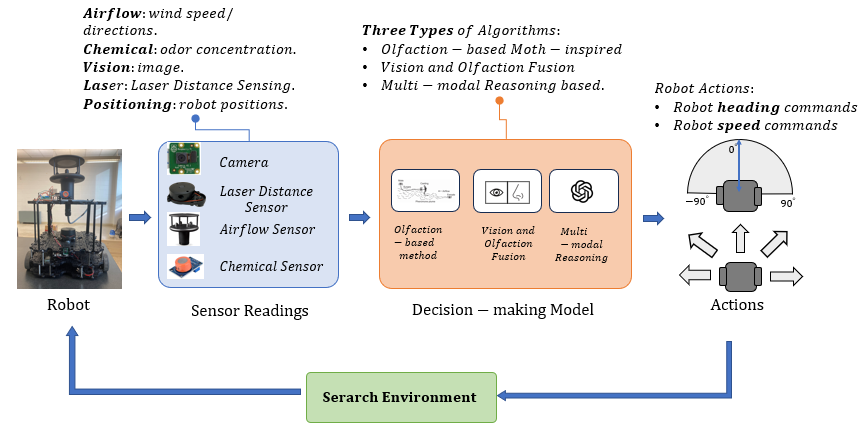
\includegraphics[width=0.99\columnwidth]{Main/Figure/objective.png}\hspace*{0.04in}
\end{center}
\vspace{-.1in}

\caption
{ROSL decision making model.}
%\end{singlespace}
\label{fig:overall_objective}
\end{figure}

Locating an unknown odor source necessitates an effective OSL algorithm to guide the robot based on sensor observations. \textcolor{black}{Figure~\ref{fig:overall_objective} shows the main decision-making loop of the ROSL system. The robot collects data from the environment using olfaction and vision sensors. In this work, the collected data is used by one of the three algorithms -}
\begin{itemize}
    \item traditional olfaction-based ROSL algorithm (detailed in chapter~\ref{chap:olfaction}).
    \item proposed vision and olfaction fusion ROSL algorithm (detailed in chapter~\ref{chap:fusion}).
    \item proposed multi-modal reasoning-based ROSL algorithm (detailed in chapter~\ref{chap:LLM}).
\end{itemize}
The navigation algorithm calculates the robot heading for localizing the odor source. The robot heading is executed by the robot, which changes its environment state. The robot again collects data and the loop continues till it localizes the odor source.

The thesis is divided into three main chapters. The main goal of chapter~\ref{chap:olfaction} is to discuss the development of a robot platform that can be used to validate a traditional ROSL algorithm. The chapter includes -
\begin{itemize}
    \item review of recent progress of ROSL research;
    \item discussion of the development of a multi-modal robot platform for real-world experimentation, and;
    \item discussion of real-world experimentation for the validation of a traditional olfaction-only ROSL navigation algorithm.
\end{itemize}

Chapter~\ref{chap:fusion} introduces a novel ROSL navigation algorithm. It proposes the incorporation of vision sensing for ROSL navigation. The chapter includes -
\begin{itemize}
    \item discussion of the limitations of traditional olfaction-based ROSL approach;
    \item discussion of the incorporation of deep-learning-based vision sensing in ROSL with the proposed vision and olfaction fusion navigation algorithm. 
    \item real-world ROSL performance comparison of traditional olfaction-only and the proposed fusion method.
\end{itemize}

Chapter~\ref{chap:LLM} proposes the application of multi-modal LLM for zero-shot ROSL navigation. The chapter includes -
\begin{itemize}
    \item discussion of the limitations of supervised vision processing.
    \item discussion of using multi-modal Large Language Model (LLM) as the zero-shot decision maker in ROSL navigation algorithm.
    \item real-world performance comparison of the validated vision and olfaction fusion navigation algorithm with a multi-modal reasoning-based navigation algorithm.
\end{itemize}

Finally, chapter~\ref{chap:conclusion} summarizes the significance of the work.

 % Introduction

%%%%%%%%%%%%%%%%%%%%%%%%%%%%%%%%%%%%%%%%%%%%%%%%%%%%%%%%%%%%%

\chapter{OLFACTION SENSING BASED ROSL ALGORITHM}\label{chap:olfaction}

\section{Introduction}
% background and problem statement
Many prior works (see ~\ref{Subsec:olfactionRelatedResearch}) only validated ROSL algorithms in simulation environments. However, simulation environments cannot always represent real-world scenarios due to the gap between simulation and real-world environments. 
This chapter discusses the development of a multi-modal robotic platform for real-world ROSL research and the implementation and evaluation of a traditional ROSL algorithm. The works covered in this chapter were published as a conference paper \cite{hassan2023multi}.

\subsection{Related Research}\label{Subsec:olfactionRelatedResearch}
% bio-inspired OSL
Designing algorithms that replicate the navigation methods of biological organisms is a common approach in robotic odor source localization research. Various organisms, regardless of their size, rely on scent to locate objects. Whether it is a bacterium navigating an amino acid gradient or a wolf tracking prey, the ability to follow odors is vital for survival.

Chemotaxis represents the simplest odor source localization strategy in biological organisms, where navigation relies solely on olfaction. For instance, bacteria demonstrate chemotaxis by altering their movement in response to changes in chemical concentration. When they encounter higher levels of an attractive chemical, their likelihood of making temporary turns decreases, resulting in straighter movement. Conversely, in the absence of a gradient or when moving away from higher concentrations, their default turning probability remains the same \cite{berg2000motile}. This straightforward algorithm allows single-celled organisms to navigate a gradient of appealing chemicals through a guided random walk. Nematodes \cite{lockery2011computational} and crustaceans \cite{radvansky2018olfactory} also utilize chemotaxis-based odor source localization. Early ROSL efforts focused on implementing such simple gradient-following chemotaxis algorithms. Typically, these methods used a pair of chemical sensors on plume-tracing robots, guiding them towards areas with higher concentration readings \cite{sandini1993gradient}. Several early studies \cite{grasso2000biomimetic, russell2003comparison, lilienthal2004experimental, ishida2005controlling} confirmed the effectiveness of chemotaxis in laminar flow environments, characterized by low Reynolds numbers. However, in turbulent flow environments with high Reynolds numbers, alternative methods inspired by more complex biological navigation techniques and engineering techniques were proposed.

Odor-gated anemotaxis navigation is a more sophisticated olfaction-based odor source localization method that uses both odor and airflow senses for navigation. Moths \cite{murlis1992odor, vickers2000mechanisms, carde2008navigational}, birds \cite{nevitt2000olfactory, wallraff2004avian}, and other organisms utilize this type of navigation. Specifically, mimicking the mate-seeking behavior of male moths led to the development of the moth-inspired method in ROSL research. This method has been successfully applied in various robotic OSL scenarios \cite{shigaki2017time}. Additionally, diverse bio-inspired search strategies such as zigzag, spiral, fuzzy-inference, and multi-phase exploratory approaches have been introduced in recent time\cite{shigaki2019modeling}. Recent bio-inspired OSL navigation methods have also aimed to increase the complexity of the search environment. For example, chemical plume tracking is performed in three-dimensional environments using three-dimensional moth-inspired OSL search \cite{rahbar20173, shigaki2022palm}.

Engineering-based methods differ from bio-mimicking algorithms by relying on mathematical models to estimate odor source locations. These approaches are often referred to as infotaxis \cite{vergassola2007infotaxis}. They involve constructing source probability maps, dividing the search area into regions, and assigning probabilities that indicate the likelihood of each region containing the odor source. Algorithms used for constructing such maps include Bayesian inference, particle filters, stochastic mapping \cite{jakuba2007stochastic}, source term estimation \cite{rahbar2019algorithm}, information-based search \cite{hutchinson2018information}, partially observable Markov decision processes \cite{hai2019underwater}, and combinations of infotaxis and the Dijkstra algorithm \cite{luong2023odor}. After predicting the odor source location, robots are then guided towards the estimated source via path-planning algorithms such as artificial potential fields and A-star \cite{pang2009reactive, wang2019chemical}.

\subsection{Objectives}\label{Subsec:mothObjectives}
The project has two main objectives:
\begin{itemize}
    \item to discuss the development of a versatile robotics platform - including robot hardware and software setup.
    \item to implement a traditional ROSL algorithm that can lead the mobile robot to the odor source in a real-world environment.
\end{itemize}


\section{Methodology}
\subsection{Hardware Setup}\label{Subec:OSLHardware}

\begin{figure}[h] %% figure

\ \\
\vspace*{-.18in}

\begin{center}
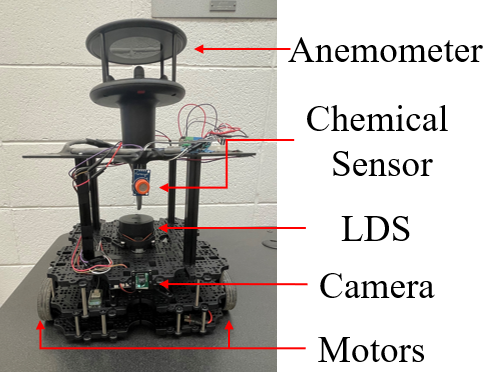
\includegraphics[width=0.6\columnwidth]{Main/Figure/olfaction_Turtlebot.png}\hspace*{0.04in}
\end{center}
\vspace{-.1in}

\caption
{The robot platform used in this work. In addition to the onboard sensors in Turtlebot3 model, the robot is equipped with a chemical sensor and an anemometer for measuring chemical concentration, wind speeds and directions.}
%\end{singlespace}
\label{fig:olfaction_robot}
\end{figure}

The Turtlebot3 mobile robot platform was utilized in this work. It comes equipped with a built-in camera, a LiDAR sensor, and a DYNAMIXEL driver for navigation. It is powered by Raspberry Pi 4. It uses Ubuntu and Robot Operating System (ROS) as operating systems. The onboard OpenCR controller enables the Turtlebot3 to be paired with additional sensors to enhance its functionality. Table~\ref{tab:sensors} lists the built-in and additional sensors used for OSL experiments. The Raspberry Pi Camera V2 was used for image capture, the LDS-02 Laser Distance Sensor for obstacle detection, the WindSonic Anemometer for measuring wind speed and direction in the body frame, and the MQ3 alcohol detector for detecting chemical plume concentration. Figure~\ref{fig:olfaction_robot} shows the final developed robotic platform.

\begin{table}[h]

\ \\

\caption{Type, name, and specification of the built-in camera, laser distance sensor, and added anemometer and chemical sensor.}
\label{tab:sensors}
\ \\
\centerline{
\begin{tabular}{|c|c|c|c|}
\hline
\textbf{Source}           & \textbf{Sensor Type}                                              & \textbf{Module Name}                                             & \textbf{Specification}                                                                                       \\ \hline
\multirow{2}{*}{Built-in} & Camera                                                            & \begin{tabular}[c]{@{}c@{}}Raspberry\\ Pi Camera v2\end{tabular} & \begin{tabular}[c]{@{}c@{}}Video Capture:\\ 1080p30, \\ 720p60 and VGA90.\end{tabular}                       \\ \cline{2-4} 
                          & \begin{tabular}[c]{@{}c@{}}Laser\\ Distance\\ Sensor\end{tabular} & LDS-02                                                           & \begin{tabular}[c]{@{}c@{}}Detection Range:\\ 360-degree.\\ Distance Range:\\ 160$\sim$8000 mm.\end{tabular} \\ \hline
\multirow{2}{*}{Added}    & Anemometer                                                        & \begin{tabular}[c]{@{}c@{}}WindSonic,\\ Gill Inc.\end{tabular}   & \begin{tabular}[c]{@{}c@{}}Speed:\\ 0--75 m/s.\\ Wind direction:\\ 0--360 degrees.\end{tabular}              \\ \cline{2-4} 
                          & \begin{tabular}[c]{@{}c@{}}Chemical\\ Sensor\end{tabular}         & \begin{tabular}[c]{@{}c@{}}MQ3 alcohol\\ detector\end{tabular}   & \begin{tabular}[c]{@{}c@{}}Concentration:\\ 25--500 ppm.\end{tabular}                                        \\ \hline
\end{tabular}

}

\ \\
\vspace{-.1in}

\end{table}

\begin{figure}[h]

\ \\
\vspace*{-.18in}

\begin{center}
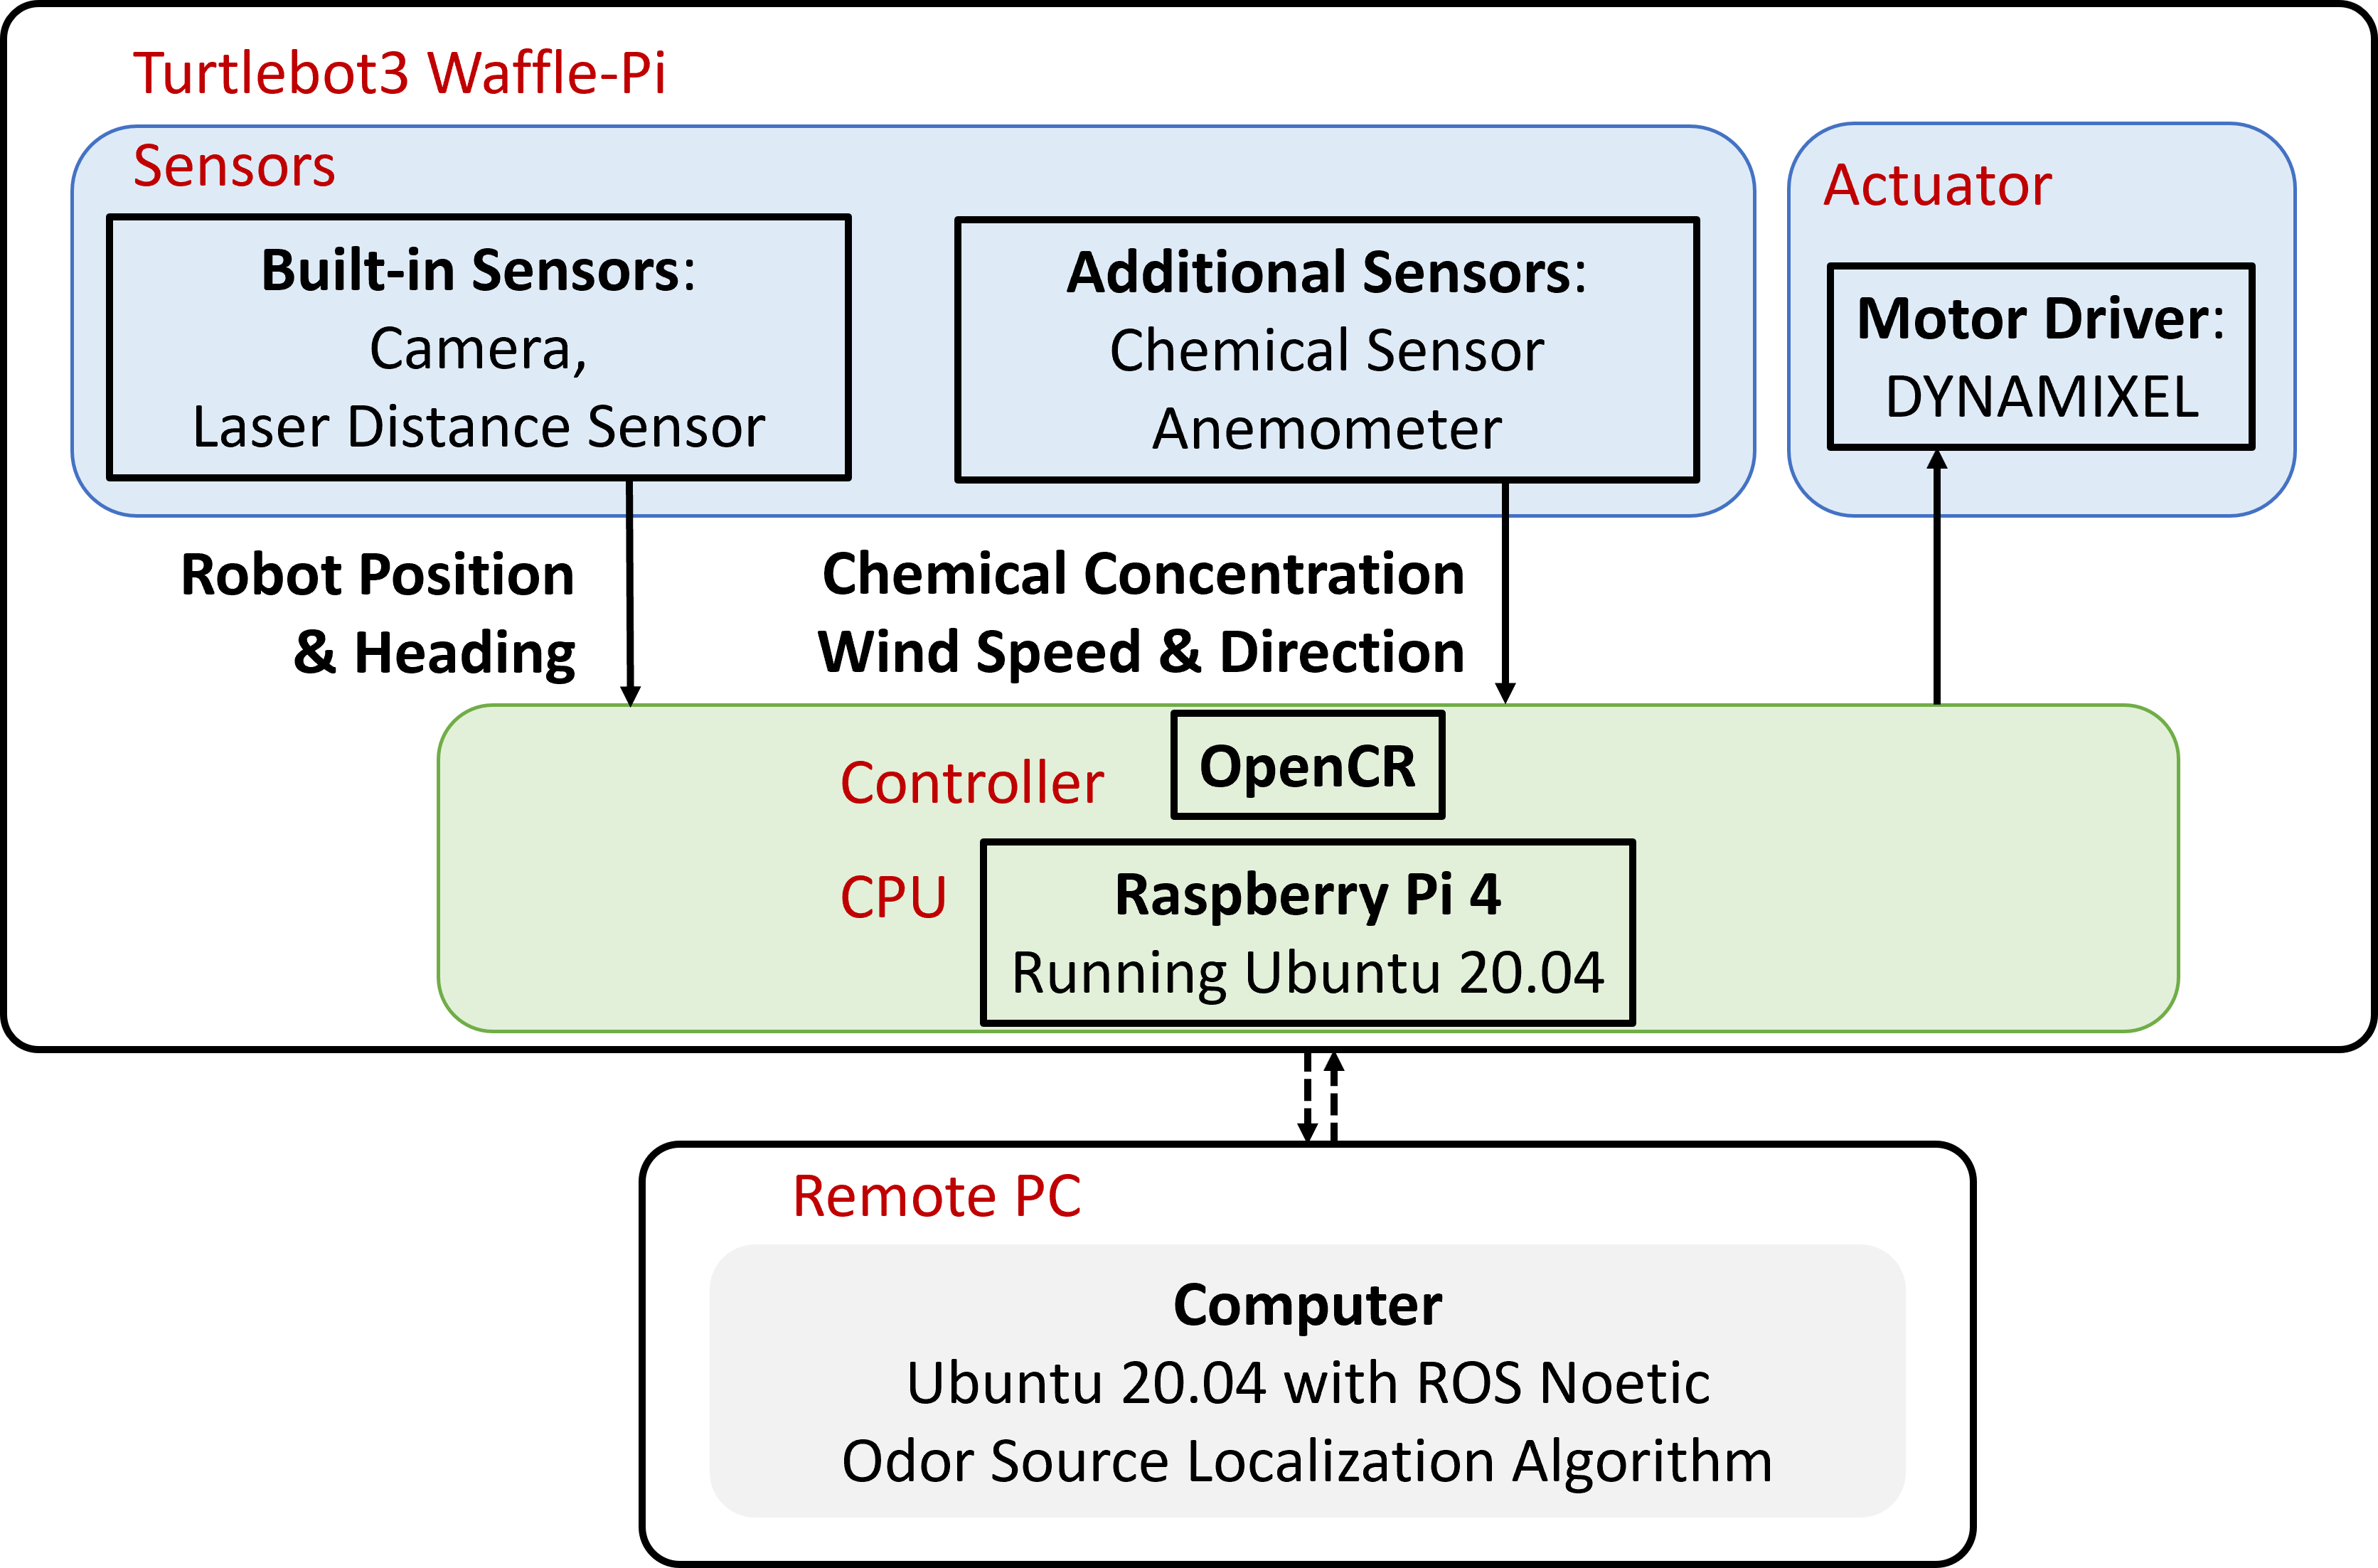
\includegraphics[width=0.9\columnwidth]{Main/Figure/hardware.png}\hspace*{0.04in}
\end{center}
\vspace{-.1in}

\caption
{System configuration. The system consists of two primary components: the Turtlebot3 and a remote PC. The solid line indicates a physical connection, while the dotted line represents a wireless link.}
%\end{singlespace}
\label{fig:OSLhardware}
\end{figure}

The Turtlebot3 features a Raspberry Pi 4 as its CPU, which has limited computing power. It runs on Ubuntu and Robot Operating System (ROS). Ubuntu provides connection capabilities with a remote computer, while ROS allows custom programs on the remote computer to subscribe to specific sensor readings from the robot and publish heading commands back to the robot in real time. ROS supports both Python and C++ programming languages. Figure~\ref{fig:OSLhardware} illustrates the proposed system configuration for the robotic system, which includes a robotic agent (Turtlebot3), an onboard controller, and a ground station (remote Personal Computer or PC). 

For this study, Ubuntu 20.04 and ROS Noetic were installed on both the robot and the remote computer to control the robot. A local area network was used to connect the robot to the remote PC.

Docker is a useful tool for ROS-based robotics research. Different version of the Robot Operating System (ROS) requires different versions of Ubuntu. Docker allows running of Ubuntu from any operating system, including Windows OS. Thus, it allows a consistent and reproducible environment for running robotics research projects.


\subsection{Moth-Inspired ROSL Algorithm}\label{subsec:moth-inspired}
Animals utilize olfaction sensing for locating unknown odor sources \cite{carde2008navigational, nielsen2015olfaction}. Wind sensing is part of animal olfactory behaviors, such as the mate-seeking behaviors of male moths \cite{murlis1992odor}, where a male moth flies against the wind direction to approach the odor source when it detects high odor concentrations. \textcolor{black}{Moth-inspired algorithm is a bio-inspired ROSL algorithm that can lead a mobile robot to an unknown odor source in the environment \cite{shigaki2017time}}.

\begin{figure}[h!]

\ \\
\vspace*{-.18in}

\begin{center}
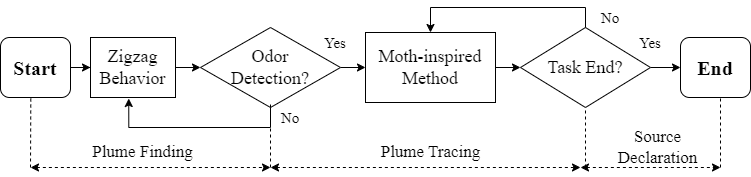
\includegraphics[width=0.7\columnwidth]{Main/Figure/olfaction_flow_diagram.png}\hspace*{0.04in}
\end{center}
\vspace{-.1in}

\caption
{The flow diagram of the proposed ROSL algorithm.}
%\end{singlespace}
\label{fig:mothinspiredFlow_diagram}
\end{figure}

Figure ~\ref{fig:mothinspiredFlow_diagram} presents the flow diagram of the proposed OSL algorithm. An OSL can be divided into three stages, including plume finding, plume tracing, and source declaration \cite{naeem2007chemical}. The first stage of the proposed algorithm is plume finding, which aims to detect plumes in the search area with crosswind 'zigzag' search \cite{wang2022robotic} since the robot has a higher chance to detect odor plumes with crosswind movements than upwind excursions. The robot turns after reaching boundaries and switches to the plume tracing stage after detecting sufficient odor concentration.

In the `Plume Tracing' stage, we proposed a moth-inspired method to command the robot to search for the odor source. The proposed moth-inspired method \cite{farrell2005chemical} can be summarized as the `surge' and `casting' behaviors, as presented in Fig. \ref{fig:olfactionSurgeCasting}. 

\begin{figure}[h]

\ \\
\vspace*{-.18in}

\begin{center}
    \subfigure[`Surge']{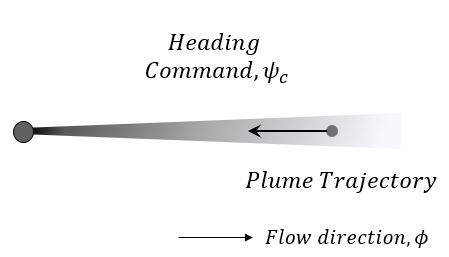
\includegraphics[width=0.4\columnwidth]{Main/Figure/olfaction_surge.png}}\hspace*{0.04in}
    \subfigure[`Casting']{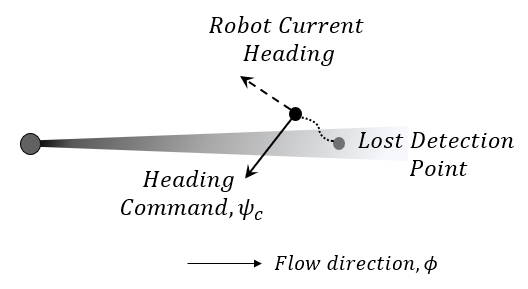
\includegraphics[width=0.4\columnwidth]{Main/Figure/olfaction_casting.png}}\hspace*{0.04in}
\end{center}
\vspace{-.1in}

\caption
{The proposed moth-inspired search behaviors in the `Plume Tracing' stage, including (a) `Surge' behavior and (b) `Casting' behavior.}
%\end{singlespace}
\label{fig:olfactionSurgeCasting}
\end{figure}

\begin{algorithm}[h!]
\caption{`Surge' Behavior}\label{alg:surge}
\begin{algorithmic}[1]
\If{Behavior is `Surge'}
    \State $\psi_{c}=\phi_{Inertial}+180$
    \If{Plume not detected, $D==0$}
        \State \Return `Track-out' Behavior
    \EndIf
\EndIf
\end{algorithmic}
\end{algorithm}

The `surge' behavior is activated when the robot detects odor plumes, i.e., $D=1$. In this behavior, i.e., Algorithm \ref{alg:surge}, the robot moves upwind to progress toward the odor source location. The heading command, i.e., $\psi_c$, in this behavior can be computed via:
\begin{equation}
    \psi_{c}=\phi_{Inertial}+180.
    \label{eqn:surge}
\end{equation}

\begin{algorithm}[h]
\caption{`Casting' Behavior}\label{alg:casting}
\begin{algorithmic}[1]
\If{Behavior is `Casting'}
    \State $\psi_{c}=\phi_{Inertial}+90$
    \If{Plume is detected, $D==1$}
        \State \Return `Surge' Behavior
    \Else
        \State \Return `Casting' Behavior
    \EndIf
\EndIf
\end{algorithmic}
\end{algorithm}

If the robot moves out of plumes, it will activate the 'casting' behavior, i.e., Algorithm \ref{alg:casting}, to move cross-wind until it finds plumes again. During this behavior, the robot uses the equation \ref{eqn:casting} to calculate the target heading $\psi_{c}$.
\begin{equation}
    \psi_{c}=\phi_{Inertial}+90.
    \label{eqn:casting}
\end{equation}
Once the robot re-detects odor plumes, it switches back to the `surge' behavior to continue the upwind movement. These two search behaviors are alternated in the `Plume Tracing' phase until the robot finds the odor source. 

\section{Experiment}\label{Sec:olfactionExperiment}
% ROSL navigation task (search area, navigation to source)
% Performance metric (type/number of tests, analysis and success matric)
\subsection{Navigation Task}\label{Subsec:fusionNavigationTask}

\begin{figure}[h] %% figure

\ \\
\vspace*{-.18in}

\begin{center}
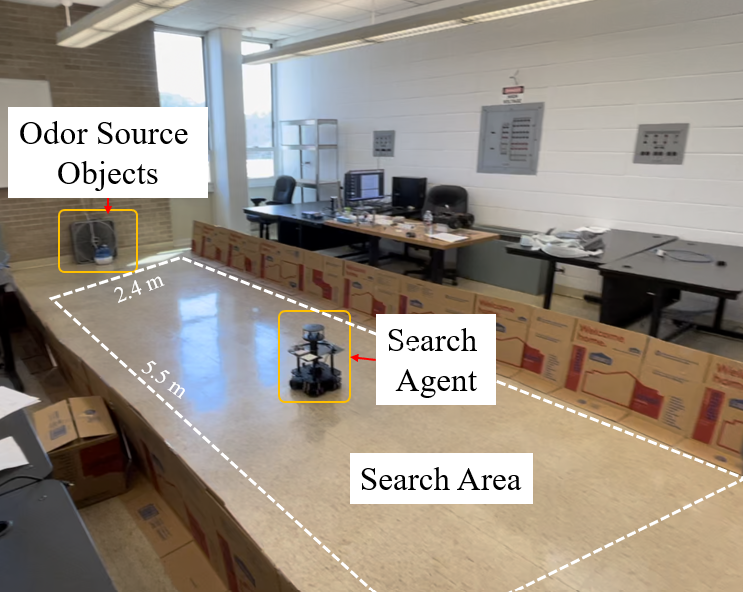
\includegraphics[width=0.9\columnwidth]{Main/Figure/olfaction_SearchArea.png}\hspace*{0.04in}
\end{center}
\vspace{-.1in}

\caption
{The experiment setup. The robot is initially placed at downwind area with the object of finding the odor source. A humidifier loaded with ethanol is employed to generate odor plumes, and an electrical fan is placed behind the humidifier to create an artificial wind field.}
%\end{singlespace}
\label{fig:olfaction_experimentSetup}
\end{figure}

The navigation experiments were conducted in the Automatic Control Lab at the Louisiana Tech University. The lab area was divided into a search area where the robot can navigate and an operation area for the remote PC. In the ROSL experiment, the mobile robot is initiated at a random position in the search area, and it use the sensor data to navigate to the odor source location. The size of the search area is $5.5 m\times2.4m$. A reference map of the search area was created using Simultaneous Localization and Mapping (SLAM). 
Ethanol vapor was used as the odor source as it is not toxic and commonly implemented in OSL research \cite{feng2019experimental}. A humidifier disperses ethanol vapor constantly as the odor plumes. An electric fan was used behind the humidifier to increase odor propagation. The robot was placed away from the odor source in this search area for each trial run. The robot utilized a chemical sensor to read plume concentration and an anemometer to read airflow speed and wind direction. Based on the sensor readings, the moth-inspired algorithm generates robot heading commands until the robot finds the odor source. In this work, the robot is considered as successfully found the odor source if the robot position is within $0.5 m$ of the odor source location.

\section{Results and Discussion}

\begin{figure}[h!] %% figure
\ \\
\vspace*{-.18in}
\begin{center}
    \subfigure{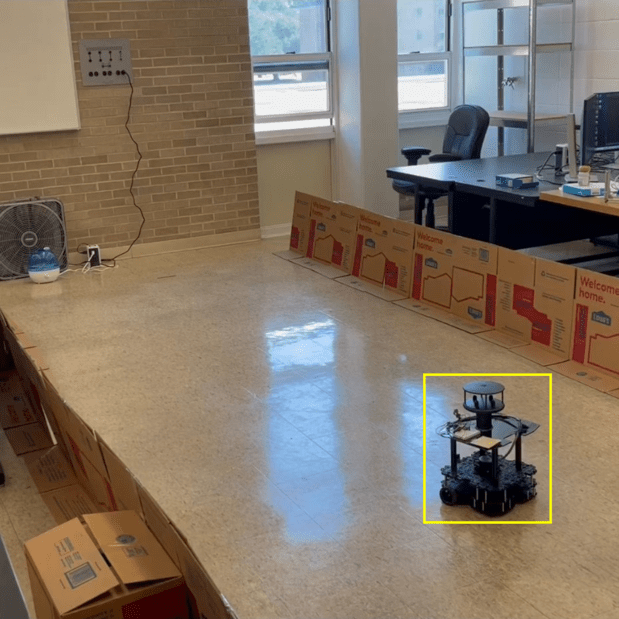
\includegraphics[width=0.33\columnwidth]{Main/Figure/olfaction_t1.png}}\hspace*{0.04in}
    \subfigure{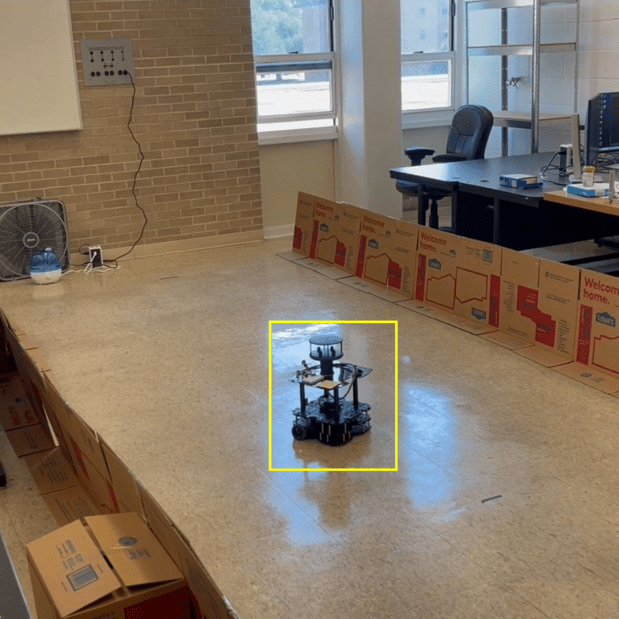
\includegraphics[width=0.33\columnwidth]{Main/Figure/olfaction_t15.png}}\hspace*{0.04in}
    \subfigure{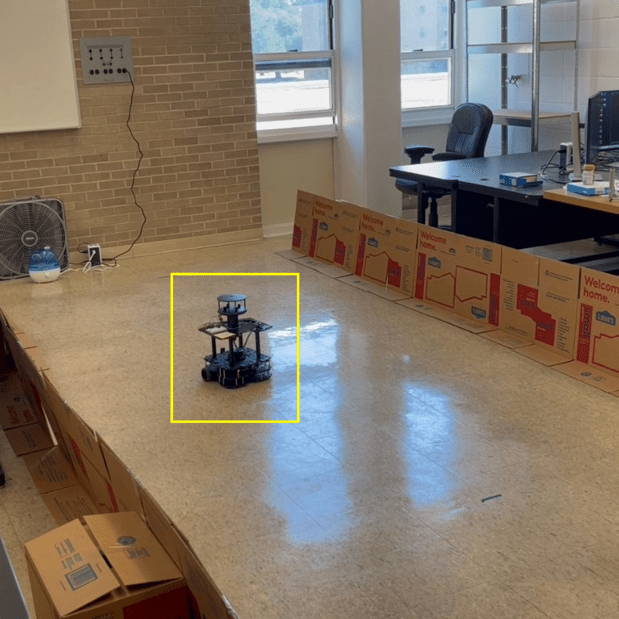
\includegraphics[width=0.33\columnwidth]{Main/Figure/olfaction_t30.png}}\hspace*{0.04in}

    \subfigure{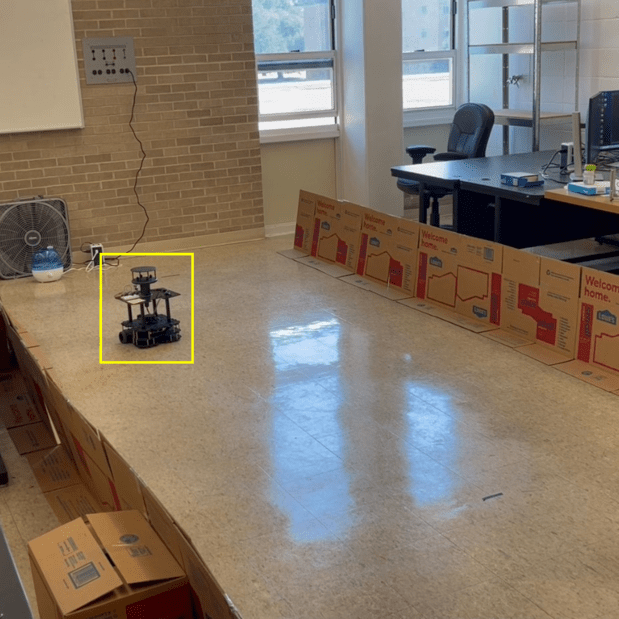
\includegraphics[width=0.33\columnwidth]{Main/Figure/olfaction_t45.png}}\hspace*{0.04in}
    \subfigure{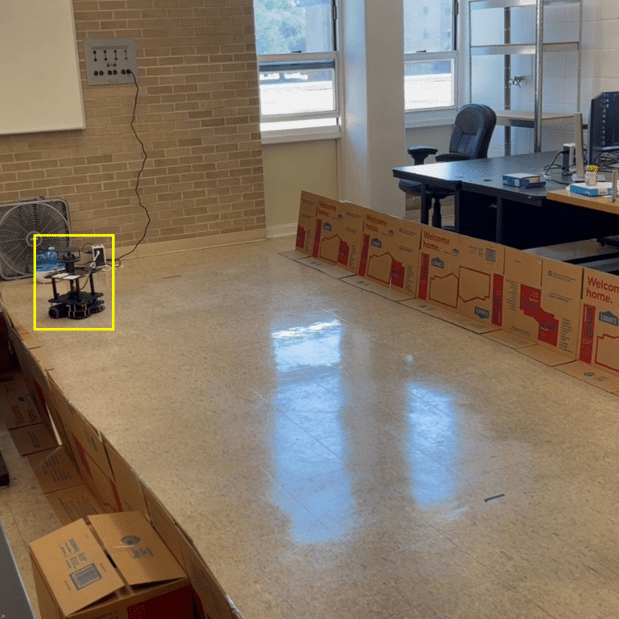
\includegraphics[width=0.33\columnwidth]{Main/Figure/olfaction_t60.png}}\hspace*{0.04in}
    \subfigure{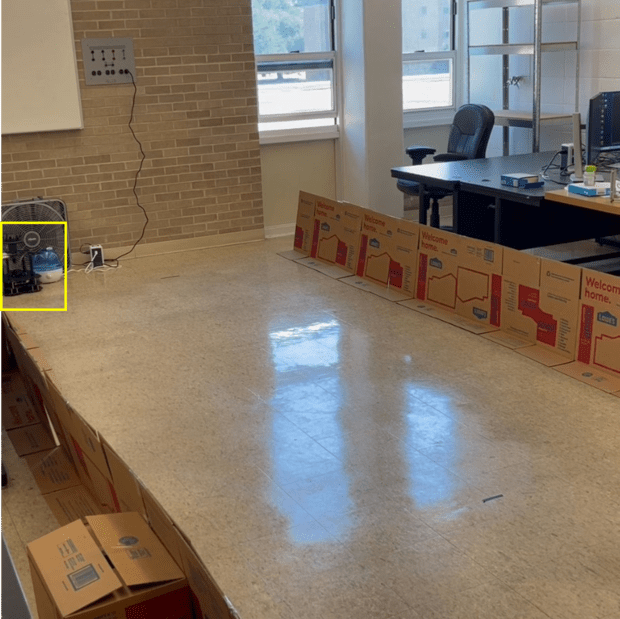
\includegraphics[width=0.33\columnwidth]{Main/Figure/olfaction_t75.png}}\hspace*{0.04in}
\end{center}
\vspace{-.1in}

\caption
{(a) Snapshots of an OSL test with the moth-inspired method. The robot position is highlighted with a yellow rectangle, and the robot correctly finds the odor source at $76$ s.}
%\end{singlespace}
\label{fig:olfaction_snapshots}
\end{figure}


Fig. \ref{fig:olfaction_snapshots} depicts Turtlebot's OSL navigation based on the moth-inspired method. At the start of the search ($t=1$ s), the robot senses odor detection and switches to the 'Plume tracing' stage to trace the odor source location. In this stage, the robot employed the `surge' behavior to move against the wind direction to approach the odor source location (from $t=1$ s to $t=15$ s). Then, the robot lost the plume contact at $t=17$ s and switched to the `casting' behavior to detect plumes in crosswind movements. At $t=30$ s, it reacquired the odor plumes and switched back to the `surge' behavior to move against the wind direction. At $t=45$ s, the robot moves close to the odor source location and remains in the `surge' behavior until it finds the odor source at $t=76$ s. The video of this trial can be found at \footnote{Experiment video link: https://youtu.be/726iJKpz1Ic}.   

The search results of the OSL trials show that the implemented moth-inspired algorithm can successfully navigate a ground mobile robot to the odor source location in a lab environment. % Thesis body starts, as many chapters as necesssary

%%%%%%%%%%%%%%%%%%%%%%%%%%%%%%%%%%%%%%%%%%%%%%%%%%%%%%%%%%%%%

\chapter{OLFACTION AND VISION SENSING BASED ROSL ALGORITHM}\label{chap:fusion}

\section{Introduction}
Traditionally, ROSL research uses olfaction data for robot navigation. Olfaction data is typically represented as the concentration level of a chemical (e.g., alcohol), and wind sensing, i.e., wind speed and direction sensing. These data have inherently less information about the odor source location. In contrast, vision data can include much more information about the location of an odor source. Thus, vision is used by most complex animals for odor source localization. 
This chapter discusses the incorporation of vision sensing in ROSL. The works covered in this chapter were published as a journal article \cite{hassan2024robotic}.

\subsection{Background}\label{Subsec:fusionBackground}
% Background (Limitation of olfaction-only) and problem statement
Chapter~\ref{chap:olfaction} shows that an olfaction-based ROSL algorithm like the moth-inspired algorithm can successfully localize odor sources in simple real-world environments with uniform laminar airflow. However in environments with complex airflow or plume distribution, olfaction-only ROSL methods can struggle to reach the odor source. Thus, while cellular organisms and simple organisms without vision (e.g., nematodes) use olfaction-based OSL \cite{lockery2011computational}, complex animals utilize multi-modal-sensing for odor source localization.

Somatosensory sensing (i.e., tactile sensing) and thermal sensing are not commonly used for finding odor sources. Vision, however, is crucial for locating the odor source \cite{kuang2014smelling}. Many different animal groups utilize vision for OSL navigation, including invertebrates such as fruit flies \cite{frye2009visually}, mosquitoes \cite{van2015mosquitoes}, beetles \cite{l2015integration}, raptors \cite{potier2019sight}, mammals, etc. Typically, vision works in conjunction with olfaction for animals to precisely identify the odor source. When animals sense high odor concentrations, they initially use vision to search for potential odor source targets. If such targets are not directly visible, they rely on reasoning and olfaction to trace odor plumes and approach the odor source. The final confirmation of the odor source usually depends on vision. Thus, both vision and olfaction are essential modalities for odor source localization.

Similarly, a robot equipped with both olfaction- and vision-sensing capabilities (e.g., a camera and a chemical sensor) should locate an unknown odor source more efficiently compared to olfaction-only OSL navigation methods. However, compared to olfaction, vision data has multiple orders of complexity. Thus, while simple analytical methods can be used to extract useful information from olfaction sensor data, extracting useful information from raw pixel values will require machine-learning-based image processing. Indeed, machine learning breakthroughs of the last decade were initiated in response to vision processing challenges. For instance, the first breakthrough CNN-based `Perceptron' model \cite{krizhevsky2012imagenet} was designed to win the ImageNet vision processing competition in 2012. After 2012, every winning project of the ImageNet competition was machine-learning based.

\subsection{Related Research}\label{Subsec:DLROSL}
Machine-learning (ML)-based methods are increasingly employed in OSL experiments. Recent advancements include the use of Deep Neural Networks (DNNs) to predict gas leak locations from stationary sensor networks and the application of reinforcement learning for plume-tracing strategies. For example, Kim et al. \cite{kim2019source} trained a Recurrent Neural Network (RNN) to predict potential odor source locations using data from stationary sensor networks obtained through simulation. Hu et al. \cite{hu2019plume} developed a plume-tracing algorithm based on model-free reinforcement learning, employing the deterministic policy gradient to train an actor-critic network for Autonomous Underwater Vehicle (AUV) navigation. Wang et al. \cite{wang2021implementation} trained an adaptive neuro-fuzzy inference system (ANFIS) to address the OSL problem in simulations, though real-world validations are needed to confirm its effectiveness.

All of these approach processes olfactory data with machine learning models. In robotics, olfaction sensors often process the concentration level or detection-rate of a chemical (e.g., alcohol). These representations inherently contain limited information about the location of the odor source. Thus, it is unclear if more complex algorithms can extract the ever-increasing amount of information from the limited olfaction data. In addition, most DL-based methods discussed above are validated in virtual environments through simulated flow fields and plume distributions, highlighting the need for real-world implementations to validate their effectiveness.

\subsection{Objectives}\label{Subsec:fusionObjectives}
This project diverges from the existing OSL navigation methods by utilizing both robotic vision and olfaction in searching for the odor source location. Olfaction-Only navigation methods often depend on airflow direction to locate the odor source, which can result in failure in turbulent airflow environments. Vision sensing can enable the robot to identify the plume source location within its visual field and approach it directly. Since visual sensing is not influenced by airflow, combining it with Olfaction-Based Navigation can help the robot better locate the odor source in turbulent airflow conditions. The core of this project is to train a deep-learning-based vision processor and to design an algorithm that integrates both vision and olfaction sensing for locating an unknown odor source location.
The objectives of this project are:
\begin{itemize}
\item to introduce vision as an additional sensing modality for ROSL. Extracting information from the vision required training of a deep-learning-based computer vision model;
\item to develop a multi-modal Vision and Olfaction Fusion Navigation algorithm with Obstacle-Avoid Navigation capabilities for ROSL tasks;
\item to compare the search performance of Olfaction-Only and Vision-Only Navigation algorithms with the proposed Vision and Olfaction Fusion Navigation algorithm in a real-world search environment with obstacles and turbulent airflow setups.    
\end{itemize}

%%%%%%%%%%%%%%%%%%%%%%%%%%%%%%%%%%%%%%%%%%%%%%%%%%%%%%%%%%%%%%%%%%%%%%%%%%%%%%

\section{Methodology}
The project introduces an efficient sensor fusion algorithm that combines vision and moth-inspired olfaction-based navigation for ROSL. To augment the capabilities of this navigation algorithm, we added obstacle avoidance capability with it. Details of the olfaction model can be found in chapter~\ref{chap:olfaction}, the deep-learning-based vision model is discussed in subsection~\ref{Subsec:fusion_vision-model}, the obstacle avoidance behavior is discussed in subsection~\ref{Subsec:obstacle-avoid}, and the proposed fusion algorithm is discussed in subsection~\ref{Subsec:fusionROSL}.

\subsection{Deep-learning-based Vision Processing Model}\label{Subsec:fusion_vision-model}
The proposed Vision-Based Navigation relies on deep-learning-based computer vision techniques. Specifically, we train a deep-learning-based object detection model, namely YOLOv7, to identify vapors emitted from the odor source. Vapors are a common and distinct feature of the odor source object, such as smoke from fire sources or chemical plumes from chemical leaks, or hydrothermal vents. It is important to note that if the odor source lacks a distinct plume feature (i.e., transparent vapors), the robot can still locate the odor source using the Olfaction-Based Navigation behavior of the proposed Vision and Olfaction Fusion algorithm. Furthermore, we provide a real-world performance comparison between Olfaction-Based Navigation, Vision-Based Navigation, and the proposed navigation algorithms.

\begin{figure}[h] %% figure

\ \\
\vspace*{-.18in}

\begin{center}
    \subfigure{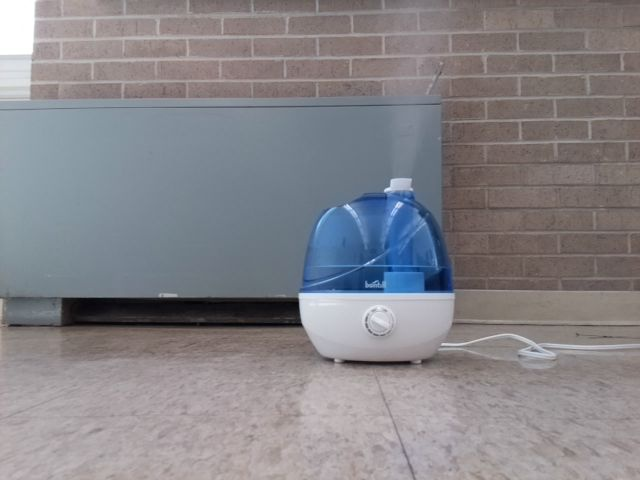
\includegraphics[width=0.5\columnwidth]{Main/Figure/visionTrainingData1.jpg}}\hspace*{0.04in}
    \subfigure{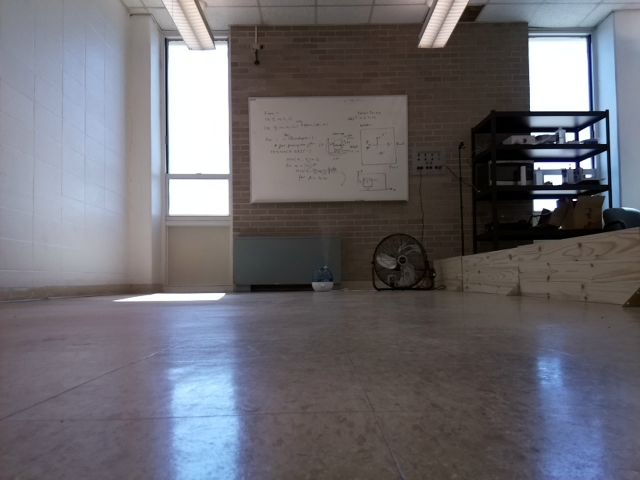
\includegraphics[width=0.5\columnwidth]{Main/Figure/visionTrainingData2.jpg}}\hspace*{0.04in}
\end{center}
\vspace{-.1in}

\caption
{Two sample frames that include humidifier odor plumes in different lighting and spatial conditions. The frames are sampled out of the total 243 frames used for training the vision model. All of the frames were captured by the Turtlebot robot in the experiment area.}
%\end{singlespace}
\label{fig:visionModelTrainingData}
\end{figure}

To generate training images for the vision model, we extracted 243 observation frames with a resolution of $640 \times 480$ while the Turtlebot was approaching the odor plumes from various angles, distances, and lighting conditions. Figure~\ref{fig:visionModelTrainingData} shows two sample frames used for training the vision model. Roboflow \cite{ciaglia2022roboflow} was used for labeling the images. This data was augmented to increase volume and was divided into training, validation, and testing datasets for model training. We used the 'Ultralytics' implementation of the YOLOv7 model, which required two hyper-parameter inputs. Epoch size of 100 and batch size of 16 resulted in a training accuracy of 98\%, and a testing accuracy of 93\%.

The implemented vision model detects if there is an odor source in the current visual frame, and if it is in the left or right part of the visual frame. In the implementation, the trained model returns the coordinates of the target object bounding box if it detects visible plume in the current visual frame. If the model detects a plume, the robot continues moving forward (i.e., $v_c=0.5$ m/s) and checks if the mid-horizontal coordinate of the bounding box is greater or less than the mid-horizontal coordinate value of the visual frame. The model took on average $1 s$ to produce output using cuda cores of RTX3060 mobile GPU of the remote computer. Thus we pass every $sr^th$ frame to the model, where $sr$ is the set value for the sensor refresh rate.

Equation~(\ref{eqn:vision_heading}) calculates the robot's heading
\begin{equation}
  \omega_c =
    \begin{cases}
       1 & \text{$0.5$ m/s if $c<\dfrac{w}{2}$}\\
      2 & \text{$-0.5$ m/s if $c>\dfrac{w}{2}$},
    \end{cases}
\label{eqn:vision_heading}
\end{equation}
where $c$ represents the horizontal midpoint of the bounding box and $w$ is the horizontal resolution of the captured image. If the bounding box is located in the left half of the image (i.e., $c < \dfrac{w}{2}$), the robot rotates left (i.e., $\omega_c = 0.5$ rad/s) to align with the plume. Otherwise, it rotates right (i.e., $\omega_c = -0.5$ rad/s) to face the plume.

\subsection{Obstacle-Avoid Navigation Behavior}\label{Subsec:obstacle-avoid}
The `Obstacle-Avoid Navigation' behavior is activated when the robot approaches an obstacle within the search environment, directing it to navigate around and avoid the obstacles. This project utilizes a Laser Distance Sensor (LDS) to sense obstacles in the surrounding area.

The proposed obstacle-avoidance behavior was derived empirically in our navigation setup. The main concept of this behavior is to determine the relative location of obstacles to the robot and command the robot to move around them. It tries to make a minimum angular change to the active direction while avoiding obstacles. The fusion algorithm avoided obstacles situated in less than $1 m$ in front - ($laser[0]$), $0.75 m$ in slightly left and right sides - ($laser[45]$) and ($laser[315]$), $0.5 m$ in left and right sides - ($laser[90]$) and ($laser[270]$). Figure~\ref{fig:laser_distance_sensing} depicts the laser distance sensing. 

\begin{figure}[h!] %% figure

\ \\
\vspace*{-.18in}

\begin{center}
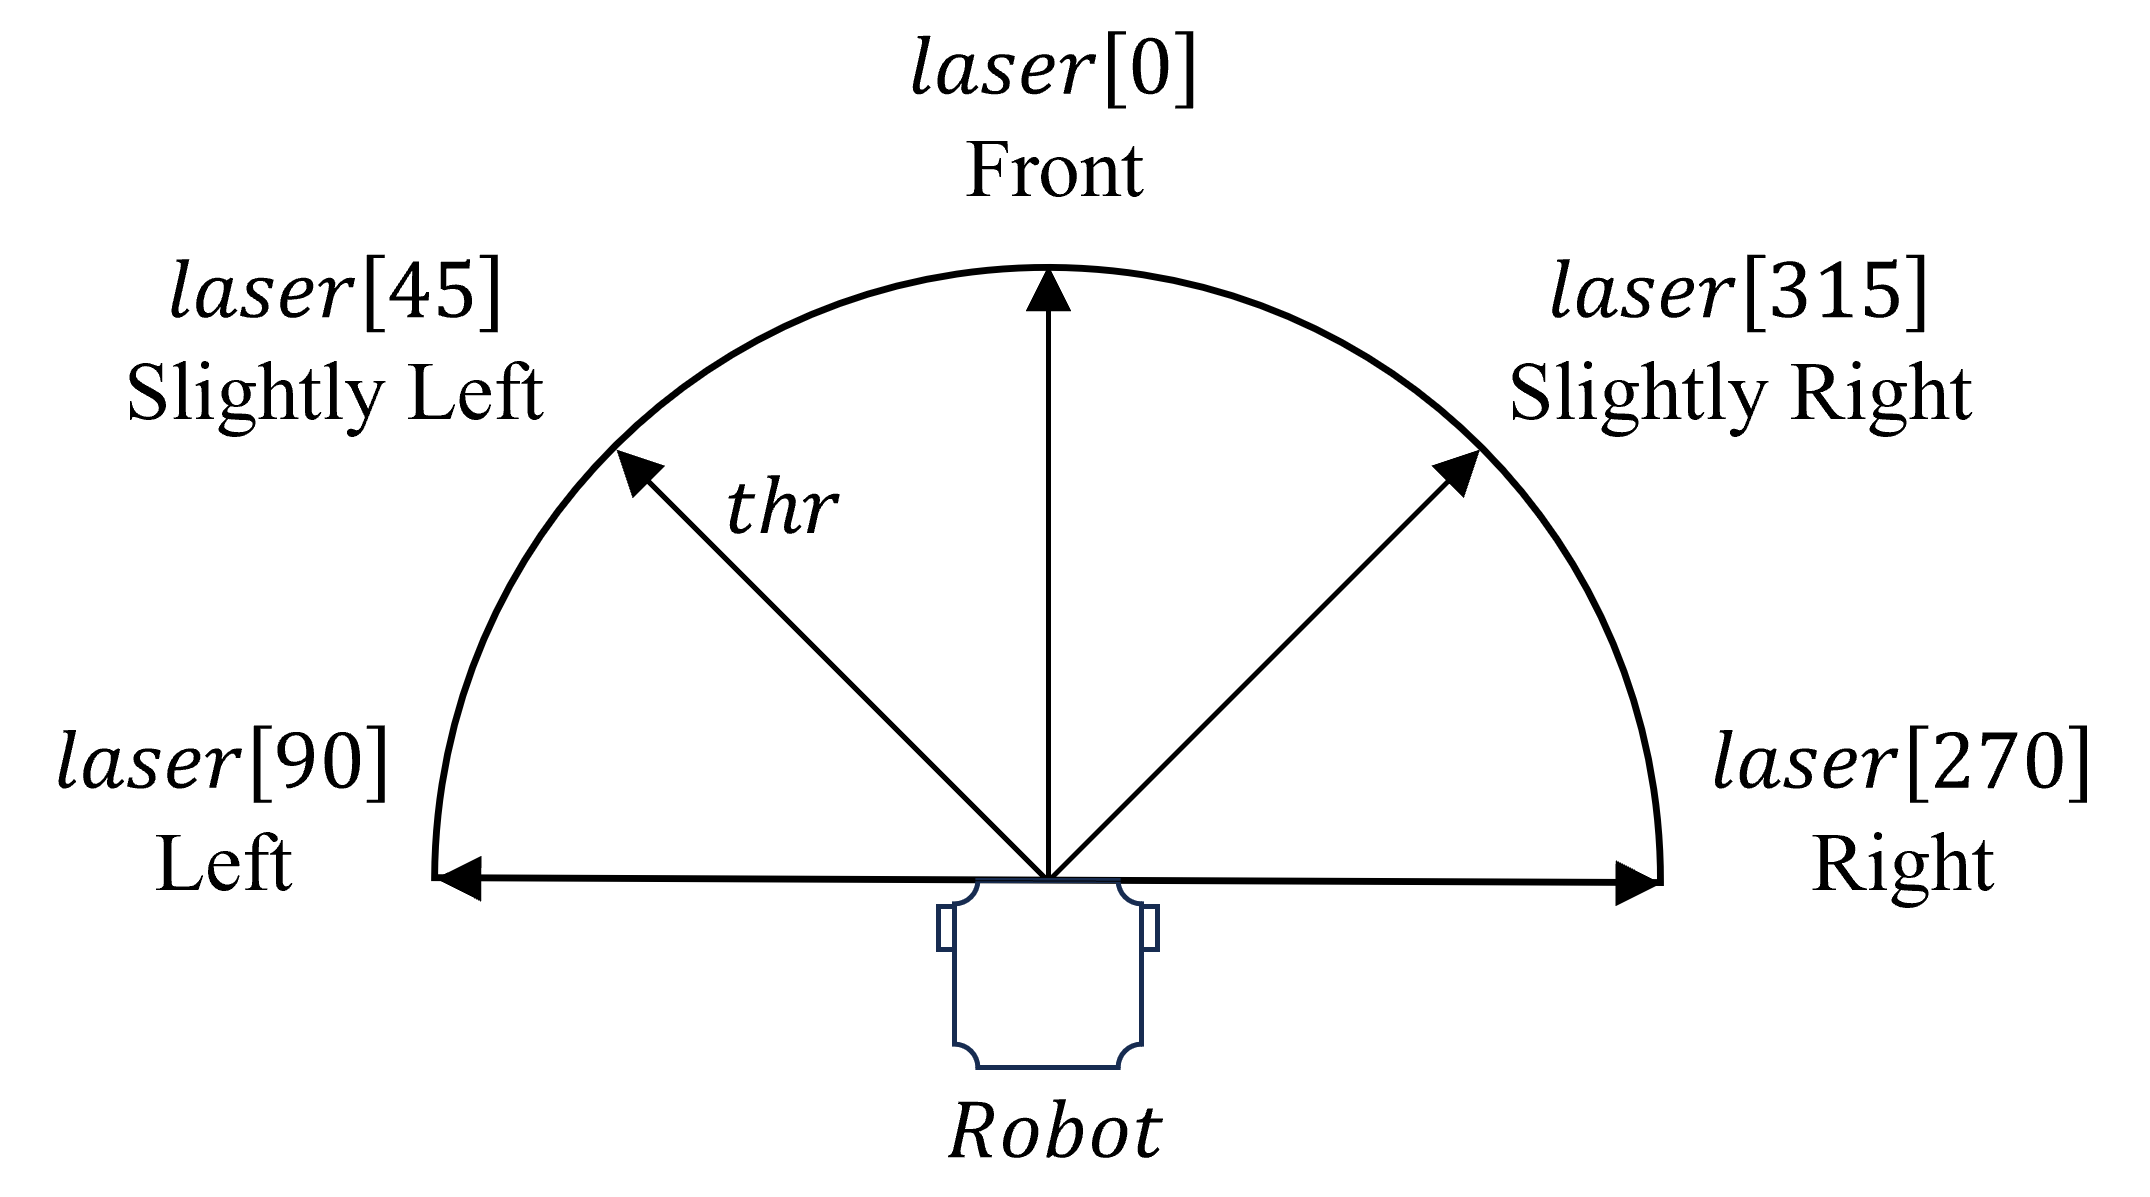
\includegraphics[width=0.7\columnwidth]{Main/Figure/robot_laserReadings.png}\hspace*{0.04in}
\end{center}
\vspace{-.1in}

\caption
{Five directions in the robot's laser distance sensing, including Left, Slightly Left, Front, Slightly Right, and Right. $laser[x]$ denotes the distance between the robot and the object at the angle $x$, which is measured from the onboard laser distance sensor.}
%\end{singlespace}
\label{fig:laser_distance_sensing}
\end{figure}


\begin{algorithm}[h!]
\caption{`Obstacle-Avoid Navigation' Behavior}\label{alg:obstacle-avoid}
\begin{algorithmic}[1]
\State Set robot linear velocity as $v_c=0.6$ m/s
\State Set robot angular velocity as $\omega_c=0$ rad/s
\If{$laser[0] > thr$}
    \State $\omega_{c}=0$ rad/s
\Else
    \State $v_c=0$ m/s and $\omega_{c}=0$ rad/s
    \If{$(laser[45]>thr)\lor (laser[315]>thr)$}
        \If{$laser[45]>laser[315]$}
            \State $\omega_{c}=0.5$ rad/s
        \Else
            \State $\omega_{c}=-0.5$ rad/s
        \EndIf
    \ElsIf{$(laser[90]>thr)\lor (laser[270]>thr)$}
        \If{$laser[90]>laser[270]$}
            \State $\omega_{c}=0.5$ rad/s
        \Else
            \State $\omega_{c}=-0.5$ rad/s
        \EndIf
    \Else
        \State $v_c=-0.5$ m/s
    \EndIf
\EndIf

\end{algorithmic}
\end{algorithm}

In the `Obstacle-Avoid Navigation' behavior \ref{alg:obstacle-avoid}, the robot continually checks for a clear path ahead, i.e., $laser[0] > thr$ (where $thr$ is the threshold for obstacle detection, set at 0.75 m in this work). If the path is clear, the robot moves forward without angular velocity, $\omega_{c} = 0$ rad/s. If the front is blocked, the robot stops and checks for clearance in Slightly Left or Slightly Right ($(laser[45] > thr) \lor (laser[315] > thr)$) directions. If either direction is clear, the robot compares the clearance between Slightly Left and Slightly Right and rotates left (i.e., $\omega_{c} = 0.5$ rad/s) or right (i.e., $\omega_{c} = -0.5$ rad/s) toward the greater clearance. If there is no clearance in either Slightly Left or Slightly Right, the robot checks for a clear path to the Left or Right ($(laser[90] > thr) \lor (laser[270] > thr)$). If a clear path exists, the robot compares the clearance between Left and Right ($laser[90] > laser[270]$) and rotates left ($\omega_{c} = 0.5$ rad/s) or right ($\omega_{c} = -0.5$ rad/s) toward the greater clearance. If all five directions are blocked, the robot moves backward ($v_c = -0.5$ m/s) to escape the dead end.

It is important to note that the proposed navigation algorithm does not have access to the global map of the search environment, the locations of obstacles, or the destination odor source. Therefore, planning-based obstacle avoidance algorithms such as the Artificial Potential Field algorithm \cite{al2022new}, A* algorithm \cite{xiang2022combined}, and Dijkstra algorithm \cite{luo2020surface} are not applicable to our problem. In such partially observable environments, using discrete behavior control is the best option. A similar approach was used in \cite{kahn2021badgr}. Compared to classic motion-planning algorithms (e.g., Dijkstra, A*, APF), our proposed obstacle avoidance algorithm has the following advantages:
\begin{itemize}
    \item It does not rely on prior knowledge of the global map, the location of obstacles, or the destination;
    \item Compared to most deep-learning-based navigation planners, it requires less inference time.
\end{itemize}


\subsection{Vision and Olfaction Fusion Algorithm}\label{Subsec:fusionROSL}

\begin{figure}[h] %% figure

\ \\
\vspace*{-.18in}

\begin{center}
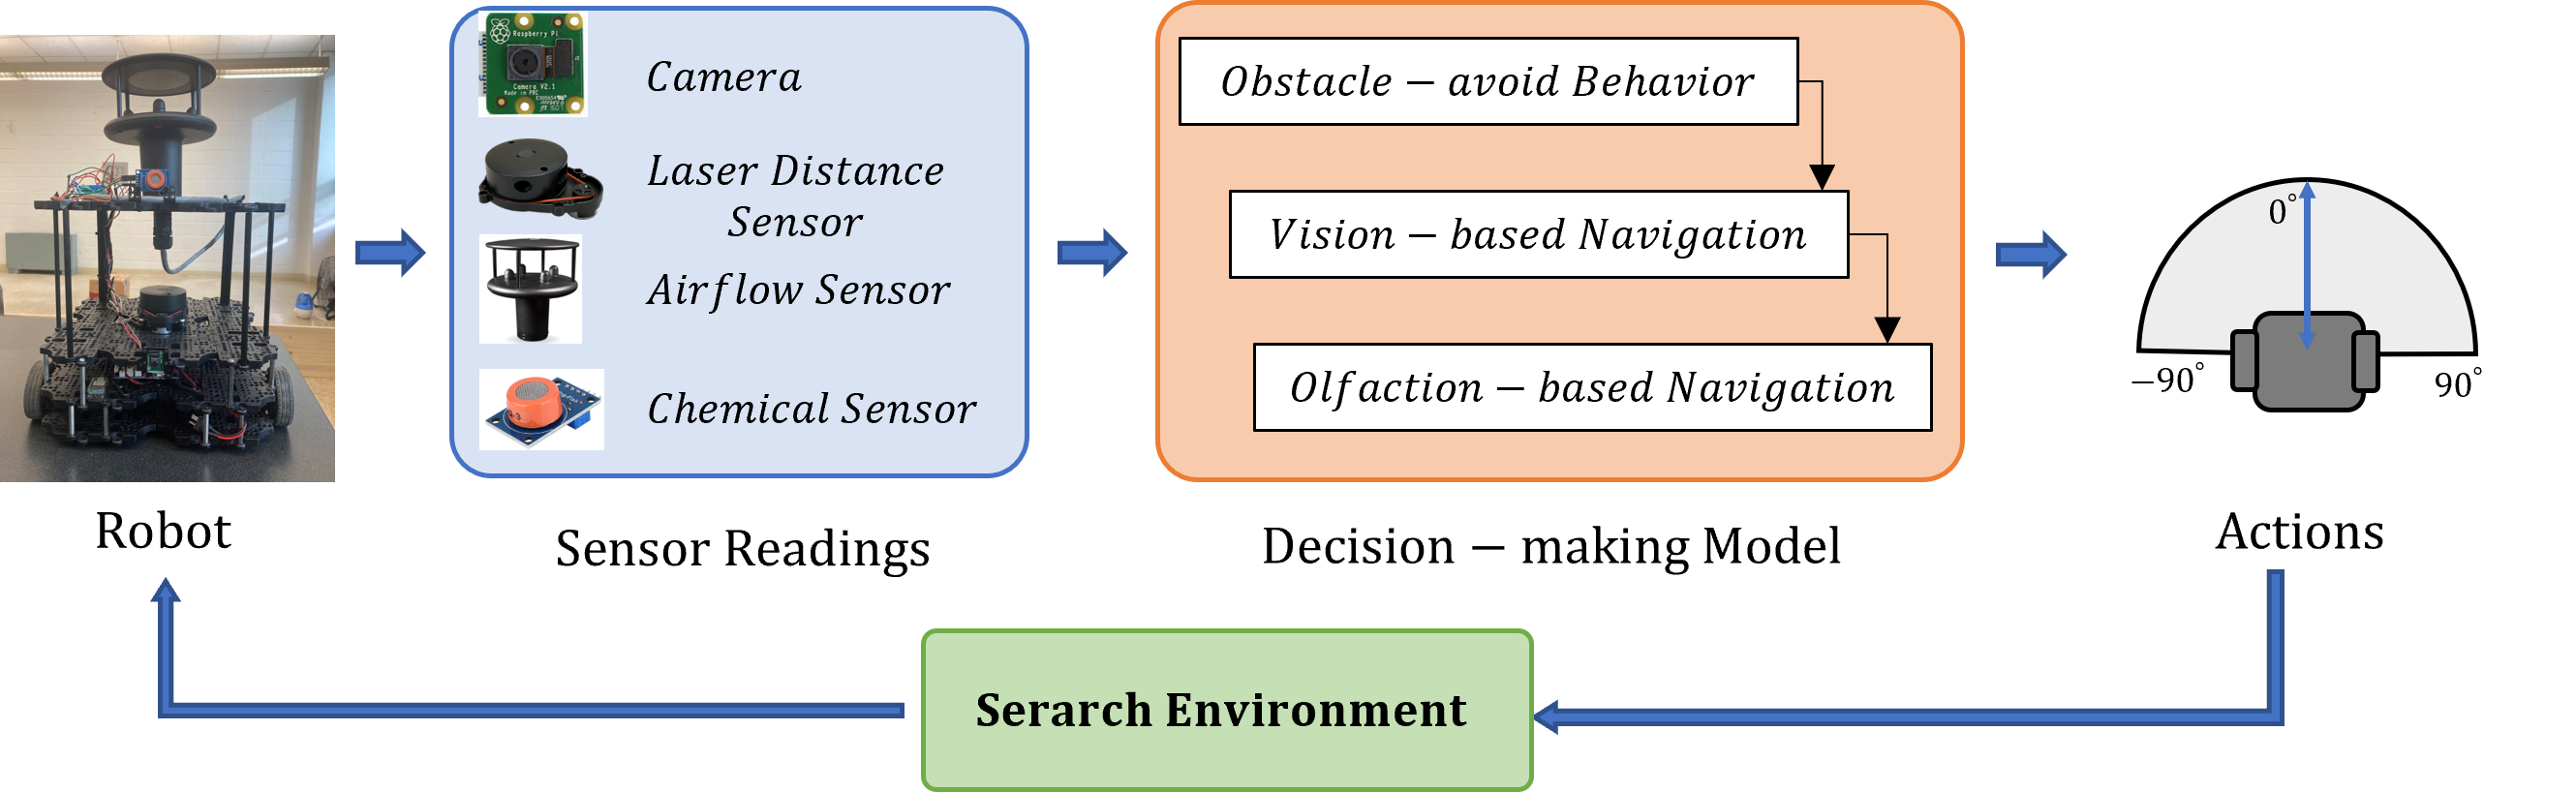
\includegraphics[width=0.7\columnwidth]{Main/Figure/OSL Model.png}\hspace*{0.04in}
\end{center}
\vspace{-.1in}

\caption
{Flow diagram of the proposed method for the OSL experiment. We employed the Turtlebot3 robot platform, outfitting it with a camera, Laser Distance Sensor, airflow sensor, chemical sensor, and other essential components. The robot uses three navigation behaviors—Obstacle-Avoid Navigation, Vision-Based Navigation, and Olfaction-Based Navigation—to determine its heading and linear velocity.}
%\end{singlespace}
\label{fig:osl_model}
\end{figure}

The proposed fusion algorithm should be able to navigate in an environment with obstacles to localize odor sources in both simple laminar and complex turbulent airflow environments. Figure~\ref{fig:osl_model} illustrates the proposed method, showcasing the developed robot platform equipped with vision and olfaction sensors. The vision sensors include a camera, while the olfaction sensors consist of a chemical detector and an anemometer. Additionally, the platform features a Laser Distance Sensing (LDS) for detecting obstacles. Vision sensor data is used by the trained YOLOv7 model to detect the presence of an odor source in the current visual frame. The output from the vision model and the raw olfaction data are transmitted to the fusion ROSL model. Based on the inputs, the model analytically determines a behavior - Obstacle-Avoid Navigation, Vision-Based Navigation, or Olfaction-Based Navigation - which is again subdivided into moth-inspired crosswind and upwind navigation. Based on the active search behavior, the algorithm calculates linear and angular heading commands. The robot then executes the heading command, gathers new sensor data at its new location, transmits it to the remote computer, and receives a new heading command - this cycle repeats until the odor source is found.

\begin{figure}[h!] %% figure

\ \\
\vspace*{-.18in}

\begin{center}
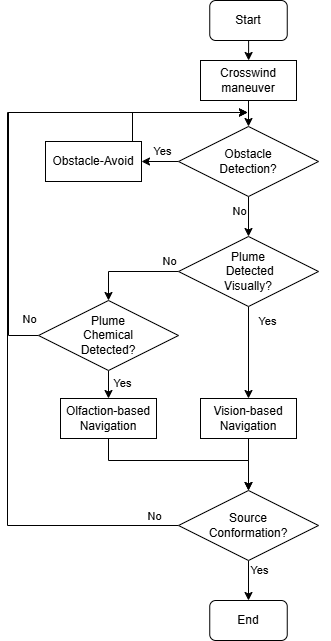
\includegraphics[width=0.5\columnwidth]{Main/Figure/FusionFlowDiagram.png}\hspace*{0.04in}
\end{center}
\vspace{-.1in}

\caption
{The flow diagram of the proposed OSL algorithm. There are four navigation behaviors, including `Crosswind maneuver', `Obstacle-Avoid Navigation', `Vision-Based Navigation', and `Olfaction-Based Navigation'.}
%\end{singlespace}
\label{fig:flow_diagram}
\end{figure}

Figure~\ref{fig:flow_diagram} illustrates the flow diagram of the proposed navigation algorithm. The fusion algorithm first checks for obstacles in the surrounding region with LDS. If there is any obstacle in the surrounding area, the algorithm activates the `Obstacle-Avoid Navigation' behavior, maneuvering the robot around the obstacles. If there are no obstacles in the surrounding area, the algorithm checks if it can sense sufficient plume concentration or valid visual detection of the plume source. In the absence of such detection, the algorithm activates the `Crosswind maneuver' behavior, moving the robot crosswind to increase the chance of detecting chemical or visual cues. During this, if a valid visual detection is obtained, the algorithm activates 'Vision-based' navigation behavior, directly moving the robot toward the odor source. If there is no visual detection, but sufficient chemical detection is recorded, the algorithm activates 'Olfaction-based' navigation behavior, sending the robot upwind. This cycle is repeated until the robot moves in the vicinity of the odor source, and the algorithm declares the source, marking the end of the search.

%%%%%%%%%%%%%%%%%%%%%%%%%%%%%%%%%%%%%%%%%%%%%%%%%%%%%%%%%%%%%

\section{Experiment}\label{Sec:fusionExperiment}

The focus of the experiment was to analyze and compare the navigation patterns of olfaction-only and vision-only navigation separately, and then then to compare the performance and navigation pattern of the fusion navigation model.

% ROSL navigation task
\subsection{Navigation Task}\label{Subsec:fusionNavigationTask}
\begin{figure}[h!] %% figure
\ \\
\vspace*{-.18in}
\begin{center}
\subfigure[Search Area]{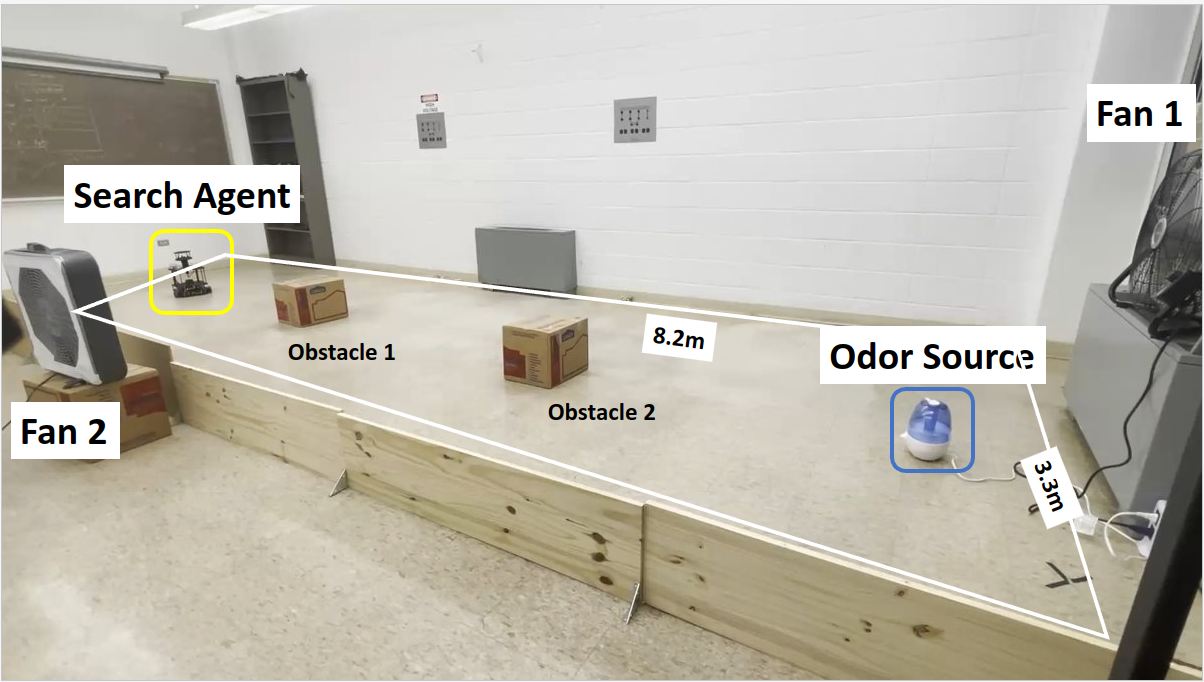
\includegraphics[width=0.55\columnwidth]{Main/Figure/Search area.png}}\hspace*{0.04in}
\subfigure[Mobile Robot]{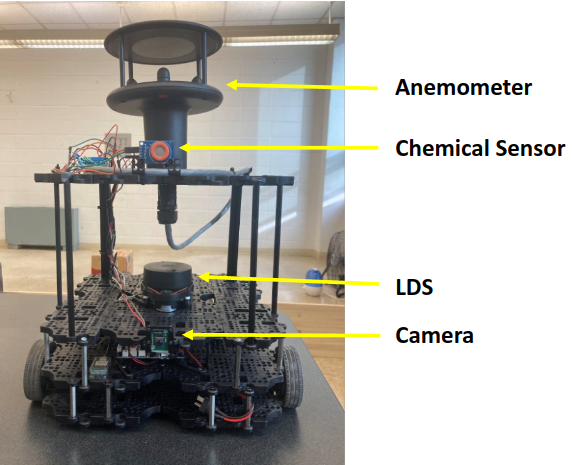
\includegraphics[width=0.4\columnwidth]{Main/Figure/mobile_robot.png}}\hspace*{0.04in}
\end{center}
\vspace{-.1in}

\caption
{(a) The experimental setup. The robot is initially placed in a downwind area with the objective of finding the odor source. A humidifier loaded with ethanol is employed to generate odor plumes. Two electric fans are placed perpendicularly to create artificial wind fields. Two obstacles are placed in the search area. {(b)} The Turtlebot3 waffle pi mobile robot is used in this work. In addition to the camera and Laser Distance Sensor, the robot is equipped with a chemical sensor and an anemometer for measuring chemical concentration, wind speeds, and directions.}
%\end{singlespace}
\label{fig:search_area_real}
\end{figure}

\begin{figure}[h!] %% figure
\ \\
\vspace*{-.18in}
\begin{center}
\subfigure[Laminar environment]{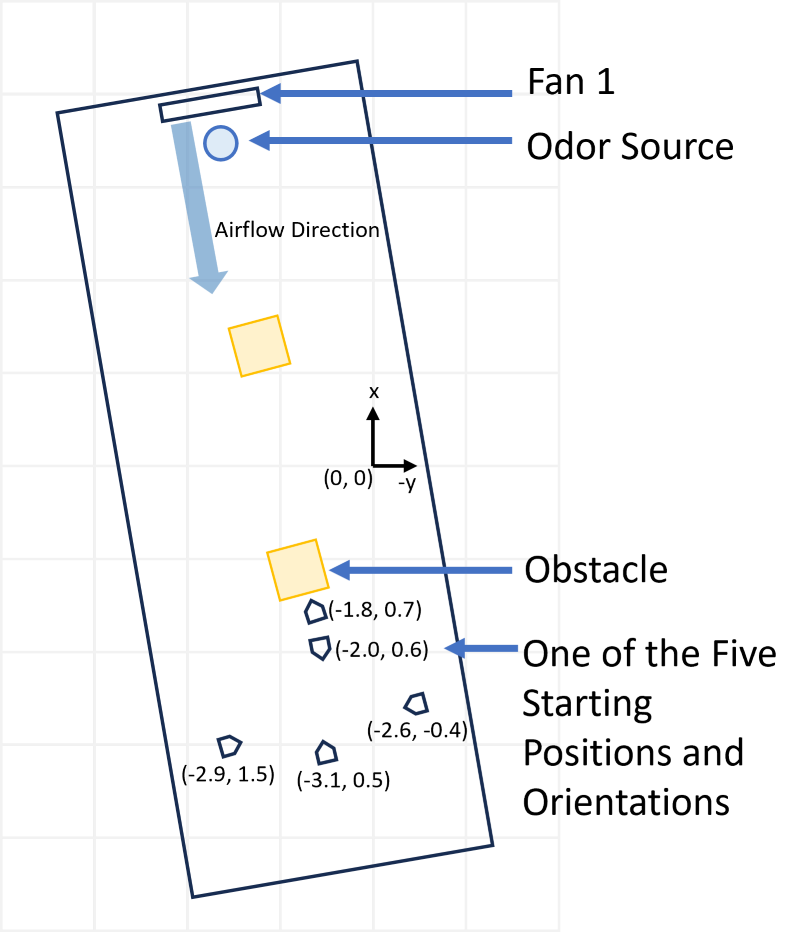
\includegraphics[width=0.4\columnwidth]{Main/Figure/Search Area Schematic Diagram e1.png}}\hspace*{0.04in}
\subfigure[Turbulent environment]{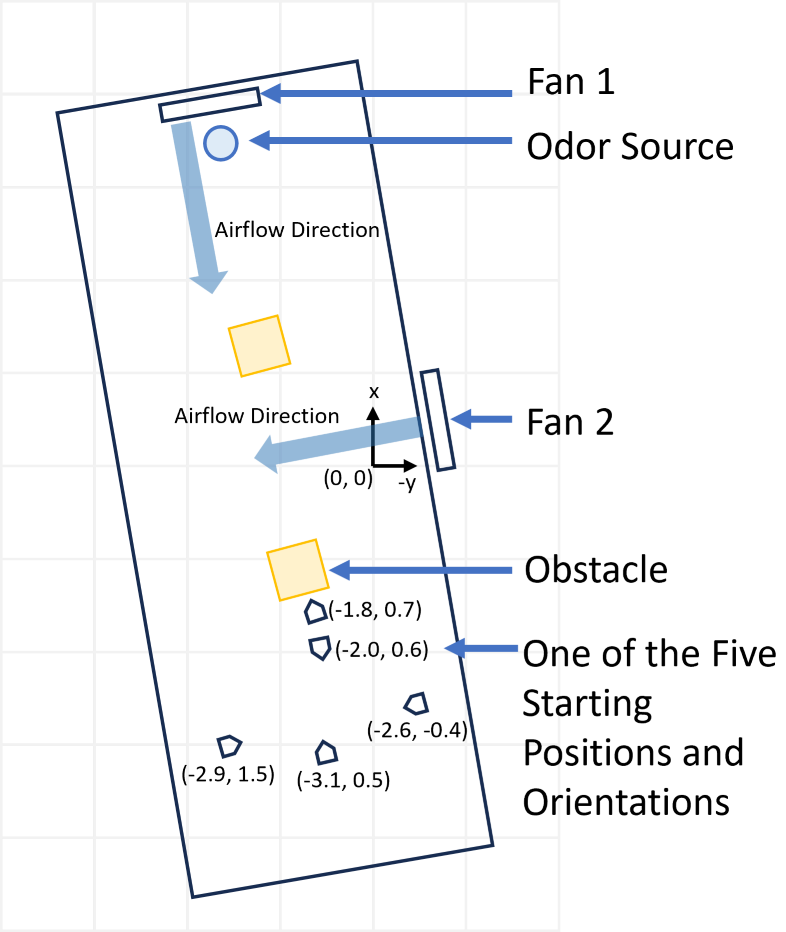
\includegraphics[width=0.4\columnwidth]{Main/Figure/Search Area Schematic Diagram e2.png}}\hspace*{0.04in}
\end{center}
\vspace{-.1in}

\caption
{The schematic diagram of the search area with e1$-$laminar airflow setup. The five robot starting positions are used for testing the performance of the Olfaction-Based Navigation, Vision-Based Navigation, and Vision and Olfaction Fusion Navigation tests. {(b)} The schematic diagram of the search area with e2$-$turbulent airflow setup.}
\label{fig:demonstration}
\end{figure}

The ROSL navigation task is similar to the one discussed in section~\ref{Sec:olfactionExperiment}. The robot will be initiated at one of the pre-determined starting positions in the search area, and it use the sensor data to navigate to the odor source location. Figure~\ref{fig:search_area_real}(a) shows the two-dimensional 8.2 m $\times$ 3.3 m search area, and the Figure~\ref{fig:search_area_real}(b) shows the robot platform. The robot platform development was detailed in subsection~\ref{Subec:OSLHardware}.

Two obstacles were placed in the search area to simulate a complex real-world search environment. The obstacles served some important purposes: 1) to test obstacle avoidance capability, 2) to block initial plume vision from the robot, 3) to further impact airflow, etc. The fans were placed to create both laminar and turbulent airflow environments in the search area. In laminar flow environments, only one fan was employed, and it was placed behind the odor source to accelerate the plume diffusion rate and create a unified wind direction field as presented in Figure\ref{fig:demonstration}{(a)}). In turbulent flow environments, we used two fans and placed them at perpendicular positions to create a mixed and turbulent wind field (as presented in Figure \ref{fig:demonstration}{(b)}).


\subsection{Reference Olfaction-only and Vision-only Algorithms}\label{subsec:fusionReferenceAlgorithms}

We designed two different navigation algorithms - only olfaction sensing-based navigation algorithm, and only vision sensing-based navigation algorithm. The purpose is to compare their navigation pattern and ROSL success rates. They were further compared with the proposed Fusion Navigation Algorithm.

\begin{figure}[h!] %% figure
\ \\
\vspace*{-.18in}
\begin{center}
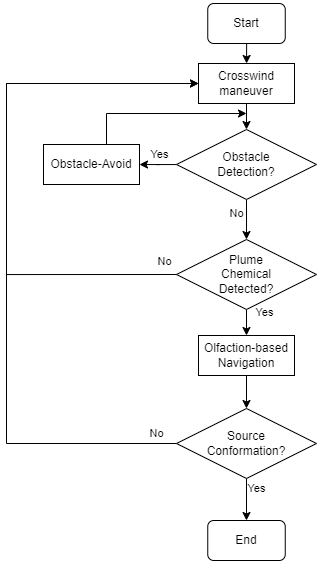
\includegraphics[width=0.4\columnwidth]{Main/Figure/OlfactionFlowDiagram.png}\hspace*{0.04in}
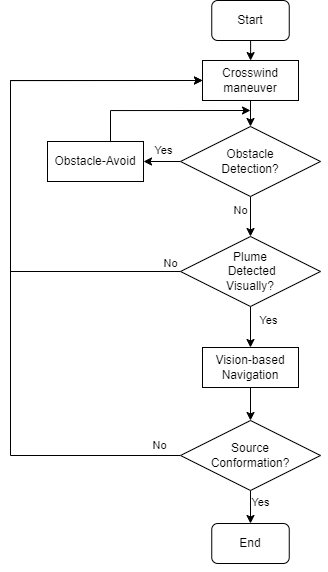
\includegraphics[width=0.4\columnwidth]{Main/Figure/VisionFlowDiagram.png}\hspace*{0.04in}
\end{center}
\vspace{-.1in}

\caption
{(a) The flow diagram of the Olfaction-Only Navigation algorithm. There are three navigation behaviors, including `Crosswind maneuver', `Obstacle-Avoid Navigation', and `Olfaction-Based Navigation'. {(b)} The flow diagram of the Vision-Only Navigation algorithm. There are three navigation behaviors, including `Crosswind maneuver', `Obstacle-Avoid Navigation', and `Vision-Based Navigation'.}
\label{fig:comparisonAlgorithm}
\end{figure}


Figure~\ref{fig:comparisonAlgorithm}(a) shows the Olfaction-Only Navigation algorithm. The algorithm first checks for obstacles in the surrounding region with LDS. If there is any obstacle in the surrounding area, the algorithm activates the `Obstacle-Avoid Navigation' behavior, maneuvering the robot around the obstacles. If there are no obstacles in the surrounding area, the algorithm checks if it can sense sufficient plume concentration. In the absence of such detection, the algorithm activates the `Crosswind maneuver' behavior, moving the robot crosswind to increase the chance of detecting chemical cues. If sufficient chemical detection is recorded, the algorithm activates 'Olfaction-based' navigation behavior, sending the robot upwind. This cycle is repeated until the robot moves in the vicinity of the odor source, and the algorithm declares the source, marking the end of the search.

Figure~\ref{fig:comparisonAlgorithm}(b) shows the Vision-Only Navigation algorithm. The algorithm first checks for obstacles in the surrounding region with LDS. If there is any obstacle in the surrounding area, the algorithm activates the `Obstacle-Avoid Navigation' behavior, maneuvering the robot around the obstacles. If there are no obstacles in the surrounding area, the algorithm checks if it can sense valid visual detection of the plume source. In the absence of such detection, the algorithm activates the `Crosswind maneuver' behavior, moving the robot crosswind to increase the chance of detecting visual cues. During this, if a valid visual detection is obtained, the algorithm activates 'Vision-based' navigation behavior, directly moving the robot towards the odor source. This cycle is repeated until the robot moves in the vicinity of the odor source, and the algorithm declares the source, marking the end of the search.

\subsection{Evaluation Metric}\label{subsec:fusionEvaluationMetric}
% Performance metric (type/number of tests, analysis and success matric)
% Real-world experimentation setup
These three algorithms were tested in two airflow environments, including the e1---laminar airflow environment and the e2---turbulent airflow environment. Thus, a total of six experimental setups were designed, i.e., three navigation methods in two airflow environments, to test the effectiveness of the proposed fusion model. Five experimental runs were conducted for each of the six experimental setups, totaling 30 trial runs. We used the same five starting positions to initialize the test runs for the three algorithms for comparability. Figure~\ref{fig:demonstration} shows the five starting positions and the two airflow setups for the experimental runs. The success rates of the three algorithms is compared to validate the effectiveness of the proposed fusion navigation algorithm.


%%%%%%%%%%%%%%%%%%%%%%%%%%%%%%%%%%%%%%%%%%%%%%%%%%%%%%%%%%%%%%%%%%%%%%%%%%%%%%55

\section{Results and Discussion}\label{Sec:fusionResult}
% trajectory graphs and result tables
% conclusion

\begin{table}[h!]

\ \\

\caption{Search time of the Vision-Only, Olfaction-Only, and Proposed Vision and Olfaction Fusion Navigation algorithms. The notation (-) indicates that the search time is beyond the limit, which is 200 seconds in this work.}
\label{tab:expeiment_result}
\ \\
\centerline{
\begin{tabular}{|c|c|c|c|c|}
\hline
\textbf{\begin{tabular}[c]{@{}c@{}}Airflow\\ Environment\end{tabular}} & \textbf{\begin{tabular}[c]{@{}c@{}}Robot\\ Initial\\ Position\\ (x, y), \\ Orientation\\ (z, w)\end{tabular}} & \textbf{\begin{tabular}[c]{@{}c@{}}Olfaction-\\ Only\\ Navigation\\ Algorithm\\ (s)\end{tabular}} & \textbf{\begin{tabular}[c]{@{}c@{}}Vision-Only\\ Navigation\\ Algorithm\\ (s)\end{tabular}} & \textbf{\begin{tabular}[c]{@{}c@{}}Vision and\\ Olfaction\\ Fusion\\ Navigation\\ Algorithm\\ (s)\end{tabular}} \\ \hline
\multirow{5}{*}{Laminar}                                               & \begin{tabular}[c]{@{}c@{}}(−2.9, 1.5),\\ (−0.6, 1.0)\end{tabular}                                            & \textbf{63.1}                                                                                     & -                                                                                           & 63.9                                                                                                            \\ \cline{2-5} 
                                                                       & \begin{tabular}[c]{@{}c@{}}(−3.1, 0.5),\\ (0.0, 35.0)\end{tabular}                                            & 71.3                                                                                              & 149.3                                                                                       & \textbf{69.9}                                                                                                   \\ \cline{2-5} 
                                                                       & \begin{tabular}[c]{@{}c@{}}(−2.6, −0.4),\\ (0.7, 0.7)\end{tabular}                                            & 74.3                                                                                              & -                                                                                           & \textbf{67.5}                                                                                                   \\ \cline{2-5} 
                                                                       & \begin{tabular}[c]{@{}c@{}}(−2.0, 0.6),\\ (1.0, −0.1)\end{tabular}                                            & \textbf{73.8}                                                                                     & -                                                                                           & 75.7                                                                                                            \\ \cline{2-5} 
                                                                       & \begin{tabular}[c]{@{}c@{}}(−1.8, 0.7),\\ (0.0, 0.1)\end{tabular}                                             & \textbf{59.1}                                                                                     & -                                                                                           & 61.1                                                                                                            \\ \hline
\multirow{5}{*}{Turbulent}                                             & \begin{tabular}[c]{@{}c@{}}(−2.9, 1.5),\\ (−0.6, 1.0)\end{tabular}                                            & -                                                                                                 & -                                                                                           & \textbf{64.0}                                                                                                   \\ \cline{2-5} 
                                                                       & \begin{tabular}[c]{@{}c@{}}(−3.1, 0.5),\\ (0.0, 35.0)\end{tabular}                                            & -                                                                                                 & -                                                                                           & \textbf{113.1}                                                                                                  \\ \cline{2-5} 
                                                                       & \begin{tabular}[c]{@{}c@{}}(−2.6, −0.4),\\ (0.7, 0.7)\end{tabular}                                            & 196.4                                                                                             & -                                                                                           & \textbf{130.7}                                                                                                  \\ \cline{2-5} 
                                                                       & \begin{tabular}[c]{@{}c@{}}(−2.0, 0.6),\\ (1.0, −0.1)\end{tabular}                                            & -                                                                                                 & 102.8                                                                                       & \textbf{131.9}                                                                                                  \\ \cline{2-5} 
                                                                       & \begin{tabular}[c]{@{}c@{}}(−1.8, 0.7),\\ (0.0, 0.1)\end{tabular}                                             & 72.3                                                                                              & -                                                                                           & \textbf{68.5}                                                                                                   \\ \hline
\end{tabular}}

\ \\
\vspace{-.1in}

\end{table}


\begin{table}[h]

\ \\

\caption{Result statistics, i.e., success rate and average search time of Vision-Based Navigation, Olfaction-Based Navigation, and the Proposed Vision and Olfaction Fusion Navigation Algorithms.}
\label{tab:expeiment_stat}
\ \\
\centerline{
\begin{tabular}{|c|c|c|c|c|}
\hline
\textbf{\begin{tabular}[c]{@{}c@{}}Navigation\\ Algorithm\end{tabular}}                     & \textbf{\begin{tabular}[c]{@{}c@{}}Airflow\\ Environment\end{tabular}} & \textbf{\begin{tabular}[c]{@{}c@{}}Success\\ Rate\end{tabular}} & \textbf{\begin{tabular}[c]{@{}c@{}}Avg.\\ Search\\ Time (s)\end{tabular}} & \textbf{\begin{tabular}[c]{@{}c@{}}Avg.\\ Travelled\\ Dist. (m)\end{tabular}} \\ \hline
\multirow{2}{*}{\textbf{Olfaction-only}}                                                    & \textbf{Laminar}                                                       & \textbf{5/5}                                                    & 68.3                                                                      & \textbf{6.1}                                                                  \\ \cline{2-5} 
                                                                                            & \textbf{Turbulent}                                                     & 2/5                                                             & 134.4                                                                     & 9.7                                                                           \\ \hline
\multirow{2}{*}{\textbf{Vision-only}}                                                       & \textbf{Laminar}                                                       & 1/5                                                             & 149.3                                                                     & 11.7                                                                          \\ \cline{2-5} 
                                                                                            & \textbf{Turbulent}                                                     & 1/5                                                             & 102.8                                                                     & 13.7                                                                          \\ \hline
\multirow{2}{*}{\textbf{\begin{tabular}[c]{@{}c@{}}Vision-Olfaction\\ Fusion\end{tabular}}} & \textbf{Laminar}                                                       & \textbf{5/5}                                                    & \textbf{67.6}                                                             & 6.2                                                                           \\ \cline{2-5} 
                                                                                            & \textbf{Turbulent}                                                     & \textbf{5/5}                                                    & \textbf{101.6}                                                            & \textbf{7.8}                                                                  \\ \hline
\end{tabular}}

\ \\
\vspace{-.1in}

\end{table}

\begin{comment}
\begin{figure}[h] %% figure

\ \\
\vspace*{-.18in}

\begin{center}
    \subfigure[e1o1]{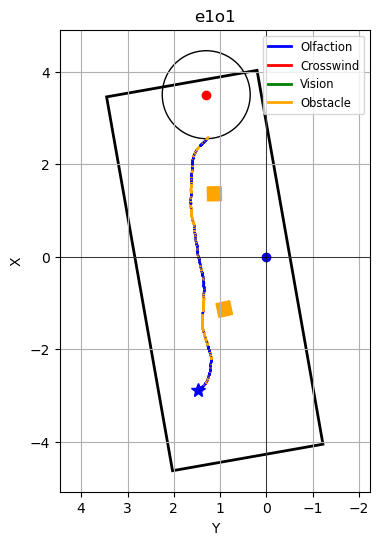
\includegraphics[width=0.2\columnwidth]{Main/Figure/e1o1.png}\label{fig:e1o1}}
    \subfigure[e1o2]{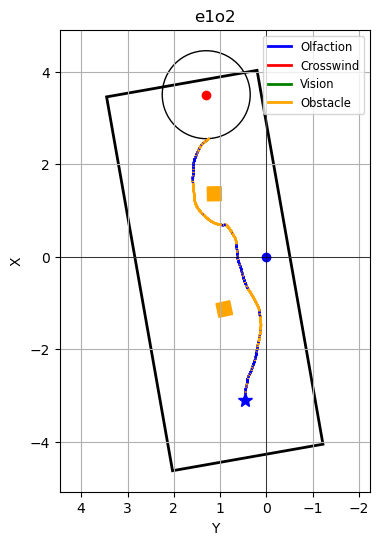
\includegraphics[width=0.2\columnwidth]{Main/Figure/e1o2.png}\label{fig:e1o2}}
    \subfigure[e1o3]{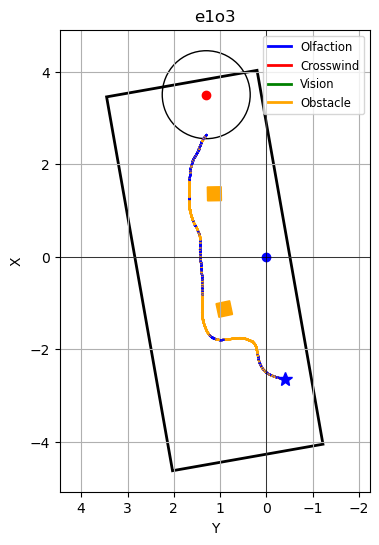
\includegraphics[width=0.2\columnwidth]{Main/Figure/e1o3.png}\label{fig:e1o3}}
    \subfigure[e1o4]{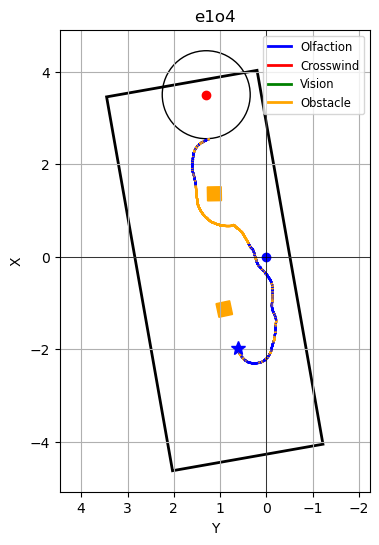
\includegraphics[width=0.2\columnwidth]{Main/Figure/e1o4.png}\label{fig:e1o4}}
    \subfigure[e1o5]{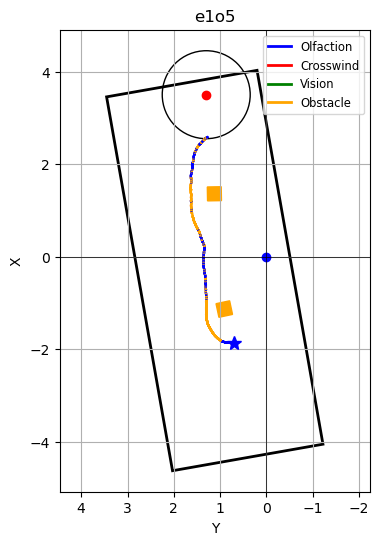
\includegraphics[width=0.2\columnwidth]{Main/Figure/e1o5.png}\label{fig:e1o5}}
    \subfigure[e2o1]{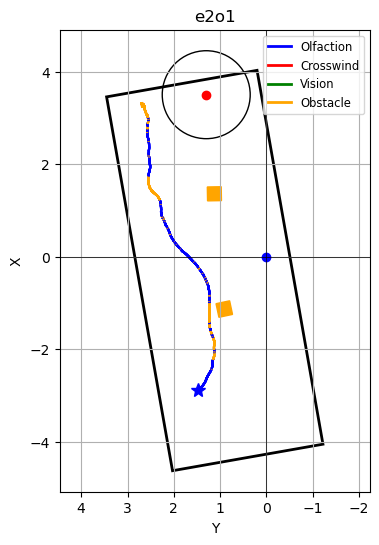
\includegraphics[width=0.2\columnwidth]{Main/Figure/e2o1.png}\label{fig:e2o1}}
    \subfigure[e2o2]{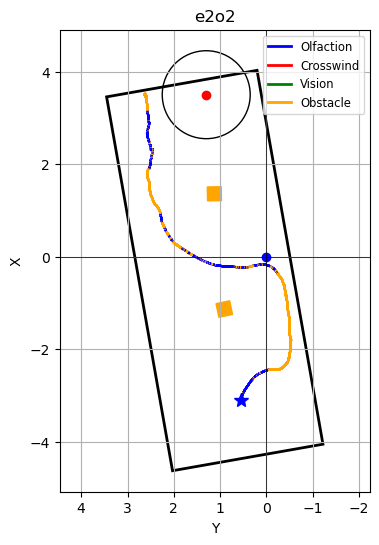
\includegraphics[width=0.2\columnwidth]{Main/Figure/e2o2.png}\label{fig:e2o2}}
    \subfigure[e2o3]{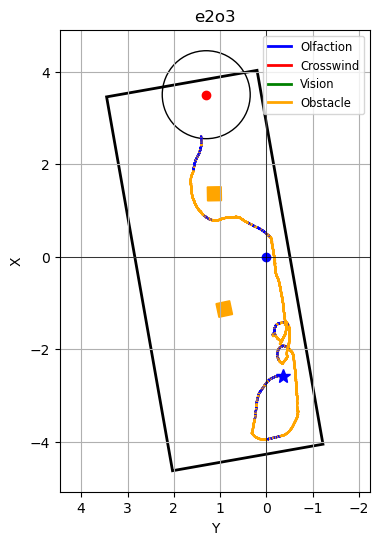
\includegraphics[width=0.2\columnwidth]{Main/Figure/e2o3.png}\label{fig:e2o3}}
    \subfigure[e2o4]{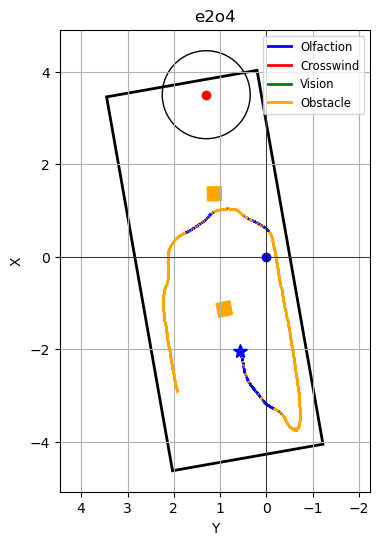
\includegraphics[width=0.2\columnwidth]{Main/Figure/e2o4.png}\label{fig:e2o4}}
    \subfigure[e2o5]{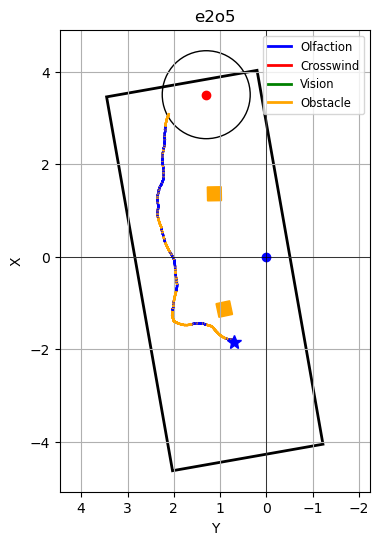
\includegraphics[width=0.2\columnwidth]{Main/Figure/e2o5.png}\label{fig:e2o5}}
\end{center}
\vspace{-.1in}

\caption
{Trajectories of OSL repeat experiments. Olfaction-only Navigation algorithm trials (o1-o5) in - (1-5) laminar airflow environment (e1), and (6-10) turbulent airflow environment (e2). The behaviors that the robot was following under the three navigation algorithms are Crosswind - crosswind maneuver behavior, Obstacle - Obstacle-avoid Navigation behavior, Olfaction - Olfaction-based Navigation behavior, and Vision - Vision-based Navigation behavior. Robot starting positions are highlighted with a blue star, the obstacles are the orange boxes, and the odor source is the red point with the surrounding circular source declaration region.}
%\end{singlespace}
\label{fig:individualTrajectoriesOO}
\end{figure}




\begin{figure}[h!] %% figure

\ \\
\vspace*{-.18in}

\begin{center}
    \subfigure[e1v1]{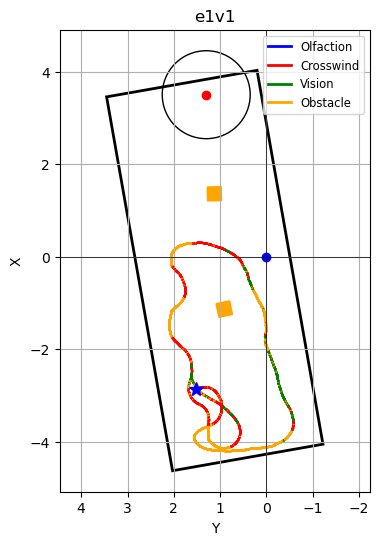
\includegraphics[width=0.2\columnwidth]{Main/Figure/e1v1.png}\label{fig:e1v1}}
    \subfigure[e1v2]{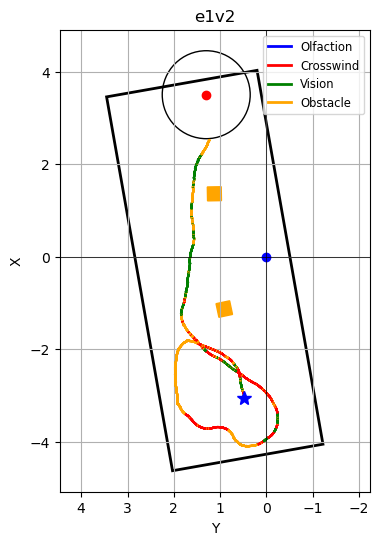
\includegraphics[width=0.2\columnwidth]{Main/Figure/e1v2.png}\label{fig:e1v2}}
    \subfigure[e1v3]{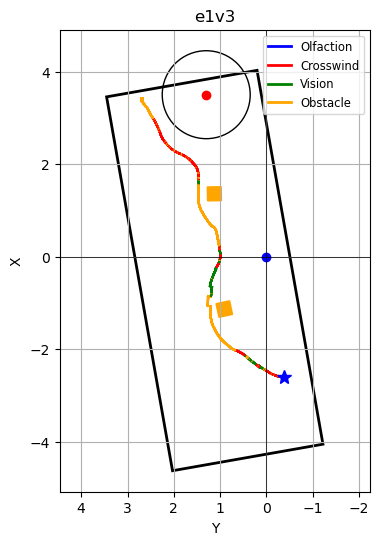
\includegraphics[width=0.2\columnwidth]{Main/Figure/e1v3.png}\label{fig:e1v3}}
    \subfigure[e1v4]{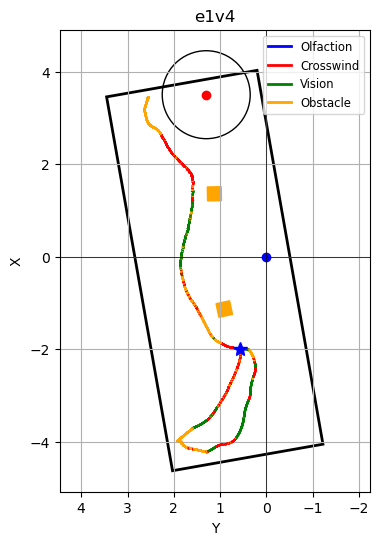
\includegraphics[width=0.2\columnwidth]{Main/Figure/e1v4.png}\label{fig:e1v4}}
    \subfigure[e1v5]{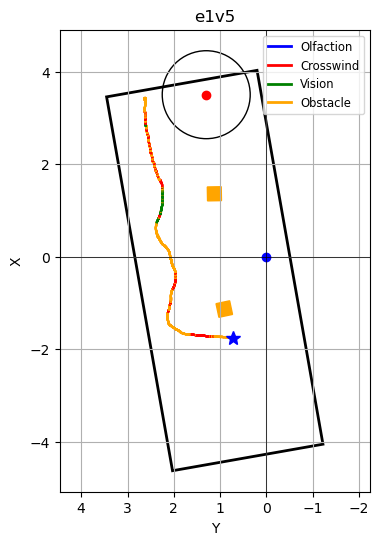
\includegraphics[width=0.2\columnwidth]{Main/Figure/e1v5.png}\label{fig:e1v5}}
    \subfigure[e2v1]{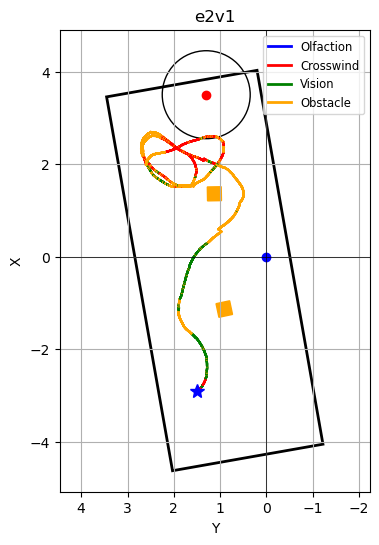
\includegraphics[width=0.2\columnwidth]{Main/Figure/e2v1.png}\label{fig:e2v1}}
    \subfigure[e2v2]{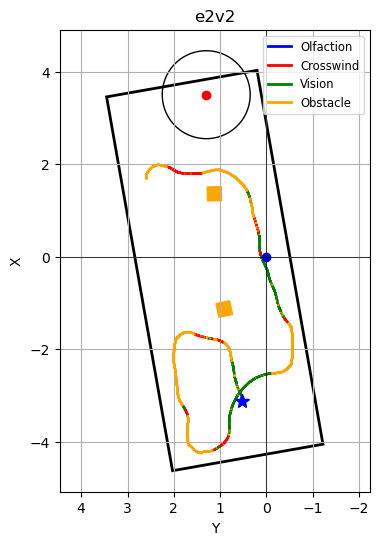
\includegraphics[width=0.2\columnwidth]{Main/Figure/e2v2.png}\label{fig:e2v2}}
    \subfigure[e2v3]{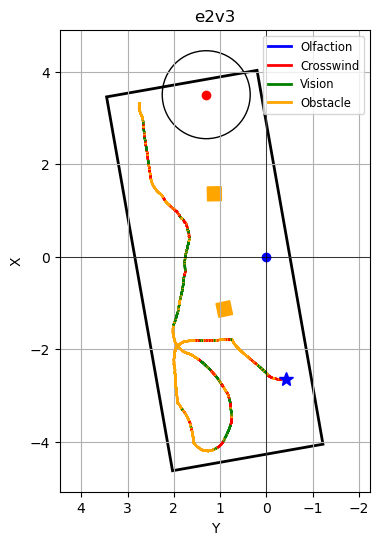
\includegraphics[width=0.2\columnwidth]{Main/Figure/e2v3.png}\label{fig:e2v3}}
    \subfigure[e2v4]{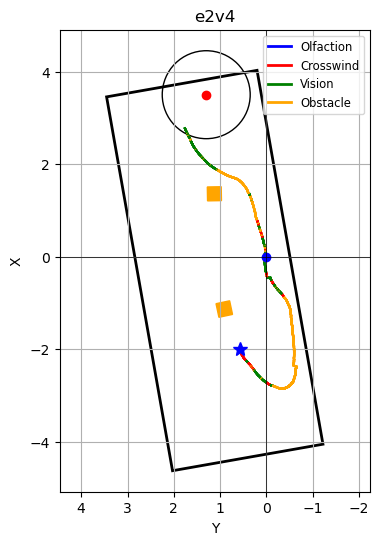
\includegraphics[width=0.2\columnwidth]{Main/Figure/e2v4.png}\label{fig:e2v4}}
    \subfigure[e2v5]{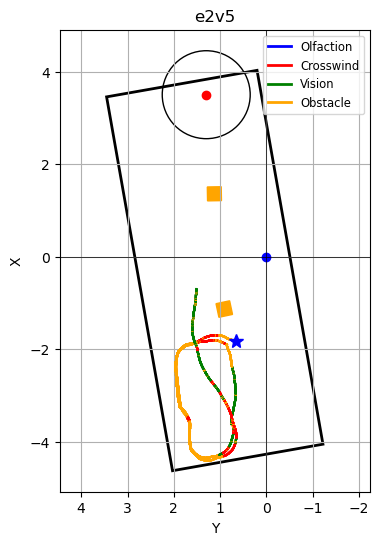
\includegraphics[width=0.2\columnwidth]{Main/Figure/e2v5.png}\label{fig:e2v5}}
\end{center}
\vspace{-.1in}

\caption
{Trajectories of OSL repeat experiments. Vision-only Navigation algorithm trials in - (1-5) laminar airflow environment (e1), and (6-10) turbulent airflow environment (e2). The behaviors that the robot was following under the three navigation algorithms are Crosswind - crosswind maneuver behavior, Obstacle - Obstacle-avoid Navigation behavior, Olfaction - Olfaction-based Navigation behavior, and Vision - Vision-based Navigation behavior. Robot starting positions are highlighted with a blue star, the obstacles are the orange boxes, and the odor source is the red point with the surrounding circular source declaration region.}
%\end{singlespace}
\label{fig:individualTrajectoriesVO}
\end{figure}



\begin{figure}[h!] %% figure

\ \\
\vspace*{-.18in}

\begin{center}
    \subfigure[e1vo1]{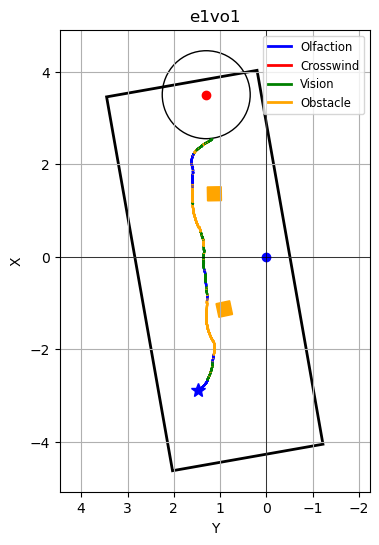
\includegraphics[width=0.2\columnwidth]{Main/Figure/e1ov1.png}\label{fig:e1vo1}}
    \subfigure[e1vo2]{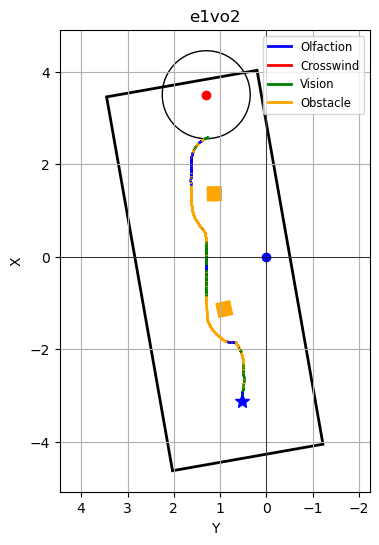
\includegraphics[width=0.2\columnwidth]{Main/Figure/e1ov2.png}\label{fig:e1vo2}}
    \subfigure[e1vo3]{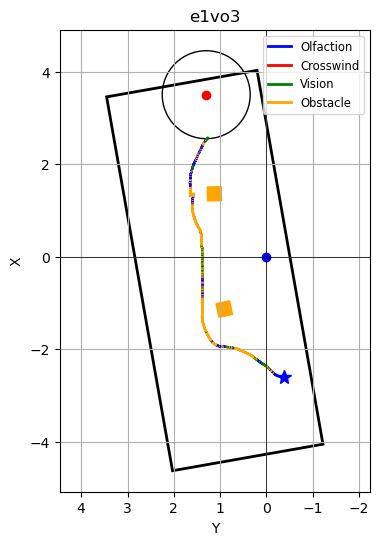
\includegraphics[width=0.2\columnwidth]{Main/Figure/e1ov3.png}\label{fig:e1vo3}}
    \subfigure[e1vo4]{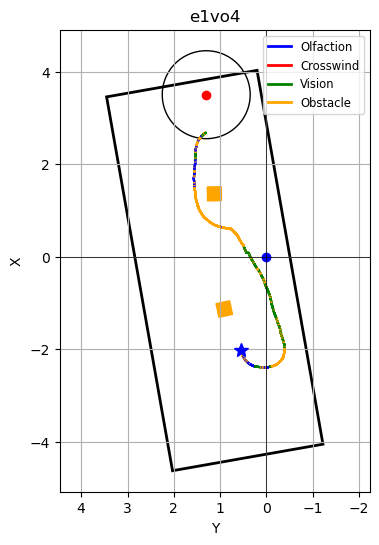
\includegraphics[width=0.2\columnwidth]{Main/Figure/e1ov4.png}\label{fig:e1vo4}}
    \subfigure[e1vo5]{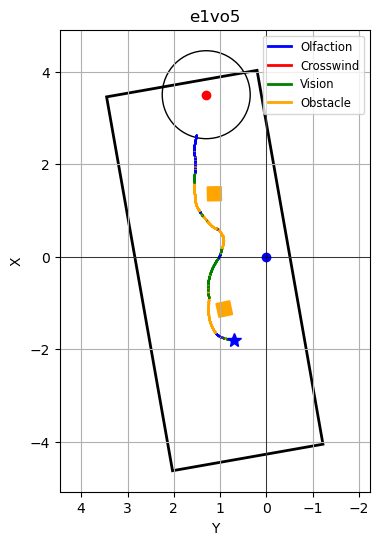
\includegraphics[width=0.2\columnwidth]{Main/Figure/e1ov5.png}\label{fig:e1vo5}}
    \subfigure[e2vo1]{\includegraphics[width=0.2\columnwidth]{Main/Figure/e2ov1.png}\label{fig:e2vo1}}
    \subfigure[e2vo2]{\includegraphics[width=0.2\columnwidth]{Main/Figure/e2ov2.png}\label{fig:e2vo2}}
    \subfigure[e2vo3]{\includegraphics[width=0.2\columnwidth]{Main/Figure/e2ov3.png}\label{fig:e2vo3}}
    \subfigure[e2vo4]{\includegraphics[width=0.2\columnwidth]{Main/Figure/e2ov4.png}\label{fig:e2vo4}}
    \subfigure[e2vo5]{\includegraphics[width=0.2\columnwidth]{Main/Figure/e2ov5.png}\label{fig:e2vo5}}
\end{center}
\vspace{-.1in}

\caption
{Trajectories of OSL repeat experiments. Vision and Olfaction Fusion Navigation algorithm trials (o1-o5) in - (1-5) laminar airflow environment (e1), and (6-10) turbulent airflow environment (e2). The behaviors that the robot was following under the three navigation algorithms are Crosswind - crosswind maneuver behavior, Obstacle - Obstacle-avoid Navigation behavior, Olfaction - Olfaction-based Navigation behavior, and Vision - Vision-based Navigation behavior. Robot starting positions are highlighted with a blue star, the obstacles are the orange boxes, and the odor source is the red point with the surrounding circular source declaration region.}
%\end{singlespace}
\label{fig:individualTrajectoriesFusion}
\end{figure}
\end{comment}

\begin{figure}[h!] %% figure
\ \\
\vspace*{-.18in}
\begin{center}
    \subfigure[e1o]{\includegraphics[width=0.3\columnwidth]{Main/Figure/e1o.png}\label{fig:e1o}}
    \subfigure[e1v]{\includegraphics[width=0.3\columnwidth]{Main/Figure/e1v.png}\label{fig:e1v}}
    \subfigure[e1vo]{\includegraphics[width=0.3\columnwidth]{Main/Figure/e1ov.png}\label{fig:e1vo}}
    \subfigure[e2o]{\includegraphics[width=0.3\columnwidth]{Main/Figure/e2o.png}\label{fig:e2o}}
    \subfigure[e2v]{\includegraphics[width=0.3\columnwidth]{Main/Figure/e2v.png}\label{fig:e2v}}
    \subfigure[e2vo]{\includegraphics[width=0.3\columnwidth]{Main/Figure/e2ov.png}\label{fig:e2vo}}
\end{center}
\vspace{-.1in}

\caption
{Robot trajectories of repeated tests in six navigation algorithm and airflow environment combinations. Trajectories in laminar airflow environments are (a) e1o—Olfaction-Only Navigation algorithm, (b) e1v—Vision-Only Navigation algorithm, and (c) e1vo—Vision and Olfaction Fusion Navigation algorithm. Trajectories in turbulent airflow environments are (d) e2o—Olfaction-Only Navigation algorithm, (e) e2v—Vision-Only Navigation algorithm, and (f) e2vo—Vision and Olfaction Fusion Navigation algorithm. The 1behaviors the robot followed: Crosswind maneuver behavior, Obstacle-Avoid behavior, Olfaction-Based behavior, and Vision-Based behavior. Five robot starting positions are marked with a blue star, obstacles are indicated by orange boxes, and the odor source is represented by a red point with the surrounding circular source declaration region.}
%\end{singlespace}
\label{fig:combinedTrajectories}
\end{figure}

Table~\ref{tab:expeiment_result} presents the run times for the 30 trial runs, consisting of 5 trials using each of the 3 navigation algorithms in the 2 airflow environments. %Figure~\ref{fig:individualTrajectoriesOO}, Figure~\ref{fig:individualTrajectoriesVO}, and Figure~\ref{fig:individualTrajectoriesFusion} illustrate the robot trajectories for each of the 30 trial runs.
Figure~\ref{fig:combinedTrajectories} shows the combined robot trajectories for the three navigation algorithms across the two airflow environments. Table~\ref{tab:expeiment_stat} summarizes the repeated test results, detailing success rate, average search time, and average distance traveled. The results indicate that the proposed Vision and Olfaction Fusion Navigation algorithm achieves the highest success rate, the lowest average search time, and the shortest average distance traveled among the three methods. This is crucial for real-world odor source localization applications, where it is essential for the robot to locate odor sources as quickly as possible.


The Olfaction-Only Navigation algorithm utilizes airflow direction to guide the robot toward the odor source. It performed well in laminar airflow environments, with the robot following relatively direct airflow paths to the odor source. However, in turbulent airflow environments, the robot was often diverted by complex airflow patterns and frequently failed to reach the odor source within the designated time limit.

Vision-Based Navigation performed poorly in both laminar and turbulent airflow environments. Due to the placement of obstacles, the robot had no initial vision of the plume from the starting position. It had to rely on Crosswind maneuver and Obstacle-Avoid Navigation behaviors until it obtained a valid plume visual. In most runs, the 200 s time limit expired before the robot could locate and navigate to the odor source.

The Vision and Olfaction Fusion Navigation algorithm test runs consistently succeeded in both laminar and turbulent airflow environments. The Crosswind maneuver and Olfaction-Based Navigation directed the robot toward the odor source, enabling it to detect the plume visually. Once the robot switched to Vision-Based Navigation, it was no longer affected by turbulent airflow.



%%%%%%%%%%%%%%%%%%%%%%%%%%%%%%%%%%%%%%%%%%%%%%%%%%%%%%%%%%%%%

\chapter{MULTI-MODAL REASONING-BASED ROSL ALGORITHM}\label{chap:LLM}

% Multimodal models
    % Biology inspiration self-supervised learning models: MIT papers
    % Brief of which brain part does what, which one processes sensory inputs, comparable DL systems
    % How LLM is a brain-inspired candidate for navigation decision by reasoning over sensory inputs.
% proposed solution: generalized reasoning over detected objects with multimodal LLM
% how multimodal model works - not just object name, but with object context.
% the model is generalized, and has the ability to solve a specific problem

% LLM as the new paradigm in robotics
    % Brief of LLM
    % why is llm good for robotics
        % from literature
        % Biology inspiration: MIT papers
            % Brief of how brain makes sensory input based navigation
                % Which  brain part does what, comparing DL systems with them
                % How LLM is a brain-inspired candidate for navigation decision by reasoning over sensory inputs.

\section{Introduction}
\subsection{Background}\label{Subsec:LLMBackground}
% background (limitation of supervised vision model) and problem statement
The Fusion navigation algorithm discussed in chapter~\ref{chap:fusion} has shown to be effective at localizing the odor source in real-world environments with turbulent airflow and a few obstacles. But the vision sensing can only extract odor source location information if the odor source emits visible plume. The vision model doesn't extract any odor source location information if visible plume is absent, or the vision is blocked. However, there is latent information in the vision data that can help narrow search boundaries. For example, we may narrow our odor source search area to a restaurant without directly seeing the odor-emitting food. However, this requires the ability to reason over the search objective and the environment. It is difficult to train a supervised vision model to gain generalized reasoning capability.

Reinforcement Learning (RL) can be used to teach an agent the relationship between the given objective and the surrounding environment \cite{sutton2018reinforcement}. However, RL requires extensive training that may be unfeasible in the real-world environments. If the agent is trained in a simulated environment, the simulation needs to closely match the complexities of the real world to ensure effective transfer of learning to the real environment \cite{zhao2020sim}. Even after sufficient training for a given objective, the learnings may not be transferable to a new objective.

In contrast to supervised and reinforcement learning, Large Language Models (LLM) have reasoning capabilities. This allows them to extract information from previously unseen data for diverse objectives. This problem of environment understanding is a central theme of embodied AI research.

% related research (embodied AI and LLM based navigation)
\subsection{Related Research}\label{Subsec:LLMRelatedResearch}

Embodied Intelligence is a growing research area focused on intelligent agents that closely interact with their environment. The field hypothesizes that intelligence emerges as a result of interacting with a challenging environment, rather than being a result of isolated computations. It gathers inspiration from diverse disciplines such as robotics, artificial intelligence, neuroscience, etc. The integration of Large Language Models (LLMs) is emerging as a new paradigm in embodied intelligence research. The embedded human knowledge and natural language processing capabilities of LLMs allow them to understand human instructions and propose solutions.

Large Language Models (LLMs) are a major milestone in the research of Natural Language Processing (NLP). LLMs are specialized models for natural language generation \cite{chowdhary2020natural}. LLMs are typically trained in self-supervised learning methods on vast internet textual data. These models follow transformer architecture \cite{vaswani2017attention}. The prominent features of this architecture include the self-attention mechanism that allows these models to find the interrelation of textual data. LLMs are achieving state-of-the-art performance in various domains including, but not limited to, natural language processing tasks \cite{naveed2023comprehensive}, robotics task planning \cite{zeng2023large}, autonomous driving \cite{cui2024survey}, etc. In the fields of robotics task planning and autonomous driving, LLMs can generate action plans based on understanding natural language instructions or representation of the environment \cite{wang2024large}. These models can make decisions in a diverse range of environments, indicating their immense potential in embodied robotics research.

To further enhance the applications of LLMs in embodied intelligence tasks, researchers are training these models with multi-modal data - like text, image, audio, etc. These models are termed as multi-modal models \cite{li2024multimodal}. Unlike supervised vision classifiers, Multimodal Lage Language Models are trained with large related vision and language data. For example, the multi-modal LLM CLIP \cite{radford2021learning} is trained to minimize the distance of related images and texts in a high-dimensional representation space. Training over massive multi-modal datasets results in rich visual reasoning ability in these models. Thus, multi-modal LLMs allow embodied AI agents to make sense of objects and events in a complex spatial environment \cite{shi2023intelligent}. Additionally, it has been shown that there are similarities between the vision understanding by mammalian brains and by self-supervised learning approach \cite{nayebi2024neural} that is utilized by LLMs. Thus, multi-modal and Large Language Models are increasingly used in visual understanding in embodied AI research. 

In recent years, a rich collection of works has been conducted in the field of LLM-based navigation. These works can be broadly categorized into planning and semantic understanding models. Planning-based methods directly generate action decisions to guide the agent. Examples of such models include Clip-Nav, NavGPT, VELMA, $A^2$Nav, MiC, etc. Semantic understanding models process sensor inputs, and the insights are then used to generate agent actions. Examples of such models include LM-Nav, L3MVN, ESC, SQA3D, etc. Table~\ref{tab:LLMapplication} briefs some of these models.

\begin{table}[h!]
\ \\
\caption{Publications on application of LLM-based algorithms for Robot Navigation}
\label{tab:LLMapplication}
\ \\
\centerline{
\begin{tabular}{|c|c|c|c|c|c|}
\hline
\textbf{Model}                                      & \textbf{Year} & \textbf{\begin{tabular}[c]{@{}c@{}}Design\\ Structure\end{tabular}} & \textbf{\begin{tabular}[c]{@{}c@{}}Training\\ Method\end{tabular}} & \textbf{Dataset}                                                   & \textbf{Application}                                                            \\ \hline
CoW                                                 & 2022          & CLIP                                                                & Zero-shot                                                          & RoboTHOR                                                           & \begin{tabular}[c]{@{}c@{}}Inddor\\ scenes\end{tabular}                         \\ \hline
ZSON                                                & 2022          & CLIP                                                                & \begin{tabular}[c]{@{}c@{}}Fine\\ tuning\end{tabular}              & MP3D                                                               & \begin{tabular}[c]{@{}c@{}}Open world\\ object-goal\\ navigation\end{tabular}   \\ \hline
LM-Nav                                              & 2022          & \begin{tabular}[c]{@{}c@{}}ViNG,\\ CLIP,\\ GPT-3\end{tabular}       & Zero-shot                                                          & \begin{tabular}[c]{@{}c@{}}Outdoor\\ environments\end{tabular}     & \begin{tabular}[c]{@{}c@{}}Outdoor\\ Navigation\end{tabular}                    \\ \hline
\begin{tabular}[c]{@{}c@{}}CLIP\\ NAV\end{tabular}  & 2022          & CLIP                                                                & Zero-shot                                                          & REVERIE                                                            & \begin{tabular}[c]{@{}c@{}}Household\\ environments\end{tabular}                \\ \hline
SQA3D                                               & 2023          & \begin{tabular}[c]{@{}c@{}}CLIP,\\ BERT,\\ GPT-3\end{tabular}       & \begin{tabular}[c]{@{}c@{}}Fine\\ tuning\end{tabular}              & ScanNet                                                            & \begin{tabular}[c]{@{}c@{}}Situated\\ question\\ answering\end{tabular}         \\ \hline
L3MVN                                               & 2023          & RoBERTa                                                             & Zero-shot                                                          & \begin{tabular}[c]{@{}c@{}}Gibson,\\ HM3D\end{tabular}             & Indoor scenes                                                                   \\ \hline
VLMAP                                               & 2023          & CLIP                                                                & Zero-shot                                                          & \begin{tabular}[c]{@{}c@{}}Matterport 3D,\\ Habitat\end{tabular}   & \begin{tabular}[c]{@{}c@{}}Navigation,\\ obstacle map\\ generation\end{tabular} \\ \hline
OVRL                                                & 2023          & \begin{tabular}[c]{@{}c@{}}ViT,\\ LSTM\end{tabular}                 & \begin{tabular}[c]{@{}c@{}}New\\ architecture\end{tabular}         & \begin{tabular}[c]{@{}c@{}}HM3D,\\ Gibson\end{tabular}             & \begin{tabular}[c]{@{}c@{}}IMAGENAV,\\ OBJECTNAV\end{tabular}                   \\ \hline
ESC                                                 & 2023          & \begin{tabular}[c]{@{}c@{}}PSL,\\ GLIP\end{tabular}                 & Zero-shot                                                          & \begin{tabular}[c]{@{}c@{}}HM3D,\\ RoboTHOR\end{tabular}           & Indoor scenes                                                                   \\ \hline
NavGPT                                              & 2023          & GPT-4                                                               & Zero-shot                                                          & \begin{tabular}[c]{@{}c@{}}R2R,\\ R2R-VLN\end{tabular}             & Indoor scenes                                                                   \\ \hline
VELMA                                               & 2023          & CLIP                                                                & \begin{tabular}[c]{@{}c@{}}Fine\\ tuning\end{tabular}              & \begin{tabular}[c]{@{}c@{}}Touchdown,\\ Map2seq\end{tabular}       & Urban VLN                                                                       \\ \hline
\begin{tabular}[c]{@{}c@{}}$A^2$\\ Nav\end{tabular} & 2023          & GPT-3                                                               & Zero-shot                                                          & \begin{tabular}[c]{@{}c@{}}R2R-Habitat,\\ RxR-Habitat\end{tabular} & \begin{tabular}[c]{@{}c@{}}Zero-shot\\ navigation\end{tabular}                  \\ \hline
MiC                                                 & 2023          & CLIP                                                                & Zero-shot                                                          & REVERIE                                                            & \begin{tabular}[c]{@{}c@{}}Remote object\\ localization\end{tabular}            \\ \hline
SayNav                                              & 2023          & GPT                                                                 & \begin{tabular}[c]{@{}c@{}}Fine\\ tuning\end{tabular}              & \begin{tabular}[c]{@{}c@{}}Habitat,\\ Gibson-4+\end{tabular}       & \begin{tabular}[c]{@{}c@{}}Multi-object\\ navigation\end{tabular}               \\ \hline
\end{tabular}
}
\ \\
\vspace{-.1in}

\end{table}

\subsection{Objectives}\label{Subsec:LLMObjectives}
The focus of this project is to use a pre-trained multi-modal LLM to perform zero-shot multi-modal reasoning for ROSL task. Specific objectives of this project are ---
\begin{itemize}
    \item to design an effective prompt for the multi-modal LLM model using the navigation goal and raw multi-modal sensory input.
    \item to design a ROSL navigation algorithm for a real-world mobile robot based on multi-modal LLM inference.
    \item to compare the search performance of the multi-modal reasoning-based ROSL algorithm with the vision and olfaction fusion navigation algorithm in a real-world search environment.
\end{itemize}

\section{Methodology}
% LLM-based algorithm
\subsection{Prompt design for the Multi-modal LLM}\label{Subsec:LLMPrompt}

\begin{figure}[h!] %% figure
\ \\
\vspace*{-.18in}
\begin{center}
    \subfigure{\includegraphics[width=0.7\columnwidth]{Main/Figure/prompt.png}\label{fig:Fprompt}}
\end{center}
\vspace{-.1in}

\caption
{The prompt used to query robot action from GPT-4o multi-modal LLM model.}
%\end{singlespace}
\label{fig:LLMPrompt}
\end{figure}

Figure~\ref{fig:LLMPrompt} shows the prompt used to query robot action from the GPT-4o model. The prompt was developed following the prompt design of the DiLu model \cite{wen2023dilu}. The Task, Action Selection Instructions, and Output Instructions stay the same for every query, only the visual frame and the olfaction reading change with the robot state.

The Task part of the prompt is to communicate the objective of the query with the LLM model. The image is passed to the model without any vision processing. The value of the plume concentration is passed as an integer value.

There are 5 robot actions that the GPT model can select - vision-based `Forward', `Right', `Left' movement, and olfaction-based `Upwind' and `Crosswind' movement. The GPT-4o model is not provided with the name of the odor source object. Rather, it must use reasoning to decide the odor source object from the rest of the objects. Additionally, it needs to utilize its vision and olfaction sensor understanding to determine the best robot action.

\begin{figure}[h!] %% figure
\ \\
\vspace*{-.18in}
\begin{center}
    \subfigure{\includegraphics[width=0.8\columnwidth]{Main/Figure/answer.png}\label{fig:Fanswer}}
\end{center}
\vspace{-.1in}

\caption
{GPT-4o chain of thought against the navigation query.}
%\end{singlespace}
\label{fig:LLMAnswers}
\end{figure}

Figure~\ref{fig:LLMAnswers} shows the outputs generated by the GPT-4o model against the navigation queries. In the first query, the GPT model can not see any potential odor source, finds the plume concentration to be lower than the threshold, and correctly selects the `Crosswind' navigation action. In the second query, the model still can not see any potential odor source, finds the plume concentration to be above the threshold, and correctly selects the `Upwind' navigation. In the third query, the odor source is visible. However, the GPT model fails to distinguish the odor source. However, it targets the fan as a potential odor source and selects the correct vision-based action `2'. Upon repeated tests, the same query also generated a wrong action decision of `4' after failing to distinguish the odor source in the visual frame. As the robot approaches closure to the odor source, the GPT model correctly distinguishes the odor source from the other objects (including the humidifier box) and selects the correct action to guide the robot to the odor source.

\subsection{Multi-modal LLM-based ROSL Navigation Algorithm}\label{Subsec:LLMROSLNav}

\begin{figure}[h!] %% figure
\ \\
\vspace*{-.18in}
\begin{center}
\includegraphics[width=0.5\columnwidth]{Main/Figure/LLMFlow.png}\hspace*{0.04in}
\end{center}
\vspace{-.1in}

\caption
{
The flow diagram of the proposed multi-modal reasoning-based navigation algorithm. There are four navigation behaviors, including `Crosswind maneuver', `Obstacle-Avoid Navigation', `Vision-Based Navigation', and `Olfaction-Based Navigation'.}
%\end{singlespace}
\label{fig:LLM_flow}
\end{figure}

Figure~\ref{fig:LLM_flow} shows the flow diagram of the multi-modal reasoning-based ROSL navigation algorithm. It shares obstacle avoidance and olfaction-based navigation functionalities with the vision and olfaction fusion navigation algorithm discussed in subsection~\ref{Subsec:fusionROSL}. However, the switching between vision and olfaction-based navigation is decided by the multi-modal LLM model.

\section{Experiment}
% ROSL navigation task (same source, platform, search area - vision/navigation-prevnting obstacles, various objects (including fake box) for reasoning, same 2 airflows)
\subsection{Navigation Task}\label{Subsec:LLMNavigationTask}

\begin{figure}[h!]

\ \\
\vspace*{-.18in}

\begin{center}
\includegraphics[width=0.9\columnwidth]{Main/Figure/LLMSearchArea.png}\hspace*{0.04in}
\end{center}
\vspace{-.1in}

\caption
{The experimental setup. The robot is initially placed in a downwind area with the objective of finding the odor source. A humidifier loaded with ethanol is employed to generate odor plumes. Two electric fans are placed perpendicularly to create artificial wind fields. An obstacle is placed in the search area. There are 5 objects to test the reasoning capability of the LLM-model.}
%\end{singlespace}
\label{fig:LLMSearchArea}
\end{figure}

The main focus of the experiment is to test the multi-modal reasoning capability of the GPT-4o multi-modal LLM. The experiments use the same search area discussed in subsection~\ref{Sec:fusionExperiment}. Figure~\ref{fig:LLMSearchArea} shows the search area used for ROSL navigation. The search area has an obstacle to block initial odor source vision - the algorithm must select appropriate olfaction-based navigation to approach the odor source at first. Once the algorithm can see the objects, the multi-modal LLM must use reason to understand which object is the valid odor source. An false target, i.e., humidifier box has been added to test the reasoning capability of the multi-modal LLM. 

% Fig~\ref{} shows the search area used for multi-modal-LLM based ROSL navigation experiments. An obstacle placed in the middle of the search area performs two function - 1) it blocks direct visual of the odor source, forcing the robot to follow initial olfaction-based navigation, 2) it tests obstacle avoidance behavior discussed in section~\ref{Subsec:obstacle-avoid}.
% The significant change in this experiment is the addition of various objects depicted in fig~\ref{}.


\subsection{Evaluation Metric}\label{subsec:LLMEvaluationMetric}
The performance of the multimodal-LLM-based ROSL navigation algorithm was compared with the vision and olfaction fusion navigation algorithm discussed in section ~\ref{Subsec:fusionROSL}. %The fusion navigation algorithm can be thought of as an analytical approach to vision and olfaction sensing based ROSL in this case. 
Section~\ref{Sec:fusionResult} showed that the fusion navigation algorithm can successfully localize the odor source using both olfaction and plume vision information. The high testing accuracy of the trained model resulted in accurate plume vision detection from various distances, angles, lighting conditions, etc. On the contrary, the multi-modal LLM model is not trained to know what the odor source object is. Given the goal of the task, the model must - 1) detect objects present in the visual frame, 2) reason from the provided goal which object is the odor source, and 3) select actions that'll guide the robot towards the odor source.

If the average ROSL performance of the multi-modal LLM-based navigation algorithm is not statistically worse than the average ROSL performance of the fusion navigation model, then the multi-modal LLM-based navigation algorithm could be considered a valid ROSL navigation algorithm.

The fusion and multi-modal LLM-based algorithm were tested starting from four positions, and four test runs were recorded from each starting position. In addition to tests conducted in laminar and turbulent airflow environments, as discussed in subsection~\ref{Subsec:fusionNavigationTask}, tests were recorded with one fan directly placed behind the humidifier, inhibiting direct visible plumes to challenge the vision sensing of the fusion and the multi-modal LLM-based algorithms. In total 48 tests were recorded to contrast the two ROSL algorithms.

\section{Results and Discussion}\label{Sec:LLMresults}
% trajectory graphs and tables
% conclusion (generalization, light platforms powered by cloud comutation, training cycle)
\begin{figure}[h!] %% figure
\ \\
\vspace*{-.18in}
\begin{center}
    \subfigure[Fusion env1 pos1]{\includegraphics[width=0.24\columnwidth]{Main/Figure/f11.png}\label{fig:Fe1p1}}
    \subfigure[Fusion env1 pos2]{\includegraphics[width=0.24\columnwidth]{Main/Figure/f12.png}\label{fig:Fe1p2}}
    \subfigure[Fusion env1 pos3]{\includegraphics[width=0.24\columnwidth]{Main/Figure/f13.png}\label{fig:Fe1p3}}
    \subfigure[Fusion env1 pos4]{\includegraphics[width=0.24\columnwidth]{Main/Figure/f14.png}\label{fig:Fe1p4}}
    
    \subfigure[LLM env1 pos1]{\includegraphics[width=0.24\columnwidth]{Main/Figure/l11.png}\label{fig:Le1p1}}
    \subfigure[LLM env1 pos2]{\includegraphics[width=0.24\columnwidth]{Main/Figure/l12.png}\label{fig:Le1p2}}
    \subfigure[LLM env1 pos3]{\includegraphics[width=0.24\columnwidth]{Main/Figure/l13.png}\label{fig:Le1p3}}
    \subfigure[LLM env1 pos4]{\includegraphics[width=0.24\columnwidth]{Main/Figure/l14.png}\label{fig:Le1p4}}
\end{center}
\vspace{-.1in}

\caption
{Robot trajectories of repeated tests in using fusion navigation algorithm (a$-$d) and multi-modal reasoning-based navigation algorithm (e$-$h) in laminar airflow environment. Four trial runs has been recorded for the four starting positions. The navigation behaviors are: Crosswind, Obstacle-Avoid, Upwind, and Vision-Based Navigation. The obstacle is indicated by orange box, and the odor source is represented by a red point with the surrounding circular source declaration region.}
%\end{singlespace}
\label{fig:LLMe1TrajectoriesLaminar}
\end{figure}

\begin{figure}[h!] %% figure
\ \\
\vspace*{-.18in}
\begin{center}
    \subfigure[Fusion env2 pos1]{\includegraphics[width=0.24\columnwidth]{Main/Figure/f21.png}\label{fig:Fe2p1}}
    \subfigure[Fusion env2 pos2]{\includegraphics[width=0.24\columnwidth]{Main/Figure/f22.png}\label{fig:Fe2p2}}
    \subfigure[Fusion env2 pos3]{\includegraphics[width=0.24\columnwidth]{Main/Figure/f23.png}\label{fig:Fe2p3}}
    \subfigure[Fusion env2 pos4]{\includegraphics[width=0.24\columnwidth]{Main/Figure/f24.png}\label{fig:Fe2p4}}
    
    \subfigure[LLM env2 pos1]{\includegraphics[width=0.24\columnwidth]{Main/Figure/l21.png}\label{fig:Le2p1}}
    \subfigure[LLM env2 pos2]{\includegraphics[width=0.24\columnwidth]{Main/Figure/l22.png}\label{fig:Le2p2}}
    \subfigure[LLM env2 pos3]{\includegraphics[width=0.24\columnwidth]{Main/Figure/l23.png}\label{fig:Le2p3}}
    \subfigure[LLM env2 pos4]{\includegraphics[width=0.24\columnwidth]{Main/Figure/l24.png}\label{fig:Le2p4}}
\end{center}
\vspace{-.1in}

\caption
{Robot trajectories of repeated tests in using fusion navigation algorithm (a$-$d) and multi-modal reasoning-based navigation algorithm (e$-$h) in turbulent airflow environment. Four trial runs has been recorded for the four starting positions. The navigation behaviors are: Crosswind, Obstacle-Avoid, Upwind, and Vision-Based Navigation. The obstacle is indicated by orange box, and the odor source is represented by a red point with the surrounding circular source declaration region.}
%\end{singlespace}
\label{fig:LLMe1TrajectoriesTurbulent}
\end{figure}


\begin{table}[h]
\caption{Comparison of Average Search Time, Travelled Distance, and Success Rate of the validated Vision and Olfaction Fusion Navigation algorithm and the proposed Multi-modal Reasoning-based Navigation algorithm.}
\label{tab:LLM_expeiment_result}
\ \\
\centerline{
\begin{tabular}{|c|c|ccc|ccc|}
\hline
\multirow{2}{*}{\textbf{\begin{tabular}[c]{@{}c@{}}Airflow\\ Env.\end{tabular}}} & \multirow{2}{*}{\textbf{\begin{tabular}[c]{@{}c@{}}Start\\ Pos.\end{tabular}}} & \multicolumn{3}{c|}{\textbf{\begin{tabular}[c]{@{}c@{}}Vision and Olfaction\\ Fusion Navigation\\ Algorithm\end{tabular}}}                                                                                                                                                    & \multicolumn{3}{c|}{\textbf{\begin{tabular}[c]{@{}c@{}}Multi-modal\\ Reasoning-based\\ Navigation\\ Algorithm\end{tabular}}}                                                                                                                                                  \\ \cline{3-8} 
                                                                                 &                                                                                & \multicolumn{1}{c|}{\textbf{\begin{tabular}[c]{@{}c@{}}Avg.\\ Search\\ Time\\ (s)\end{tabular}}} & \multicolumn{1}{c|}{\textbf{\begin{tabular}[c]{@{}c@{}}Avg.\\ Travel-\\ led\\ Dist.\\ (m)\end{tabular}}} & \textbf{\begin{tabular}[c]{@{}c@{}}Success\\ Rate\end{tabular}} & \multicolumn{1}{c|}{\textbf{\begin{tabular}[c]{@{}c@{}}Avg.\\ Search\\ Time\\ (s)\end{tabular}}} & \multicolumn{1}{c|}{\textbf{\begin{tabular}[c]{@{}c@{}}Avg.\\ Travel-\\ led\\ Dist.\\ (m)\end{tabular}}} & \textbf{\begin{tabular}[c]{@{}c@{}}Success\\ Rate\end{tabular}} \\ \hline
\multirow{4}{*}{\textbf{Laminar}}                                                & \begin{tabular}[c]{@{}c@{}}(-2.9,\\ 1.5)\end{tabular}                          & \multicolumn{1}{c|}{\textbf{72.5}}                                                               & \multicolumn{1}{c|}{\textbf{5.56}}                                                                       & \textbf{1.0}                                                    & \multicolumn{1}{c|}{75.2}                                                                        & \multicolumn{1}{c|}{5.7}                                                                                 & 1.0                                                             \\ \cline{2-8} 
                                                                                 & \begin{tabular}[c]{@{}c@{}}(-3.1,\\ 0.5)\end{tabular}                          & \multicolumn{1}{c|}{81.4}                                                                        & \multicolumn{1}{c|}{6.2}                                                                                 & 0.75                                                            & \multicolumn{1}{c|}{\textbf{80.9}}                                                               & \multicolumn{1}{c|}{\textbf{6.1}}                                                                        & \textbf{1.0}                                                    \\ \cline{2-8} 
                                                                                 & \begin{tabular}[c]{@{}c@{}}(-2.6,\\ -0.4)\end{tabular}                         & \multicolumn{1}{c|}{\textbf{89.7}}                                                               & \multicolumn{1}{c|}{\textbf{6.2}}                                                                        & 0.75                                                            & \multicolumn{1}{c|}{90.5}                                                                        & \multicolumn{1}{c|}{6.7}                                                                                 & \textbf{1.0}                                                    \\ \cline{2-8} 
                                                                                 & \begin{tabular}[c]{@{}c@{}}(-2.0,\\ 0.6)\end{tabular}                          & \multicolumn{1}{c|}{93.2}                                                                        & \multicolumn{1}{c|}{6.5}                                                                                 & 0.5                                                             & \multicolumn{1}{c|}{\textbf{74.7}}                                                               & \multicolumn{1}{c|}{\textbf{5.9}}                                                                        & \textbf{1.0}                                                    \\ \hline
\multirow{4}{*}{\textbf{Turbulent}}                                              & \begin{tabular}[c]{@{}c@{}}(-2.9,\\ 1.5)\end{tabular}                          & \multicolumn{1}{c|}{87.8}                                                                        & \multicolumn{1}{c|}{6.3}                                                                                 & \textbf{1.0}                                                    & \multicolumn{1}{c|}{\textbf{76.2}}                                                               & \multicolumn{1}{c|}{\textbf{5.6}}                                                                        & 0.75                                                            \\ \cline{2-8} 
                                                                                 & \begin{tabular}[c]{@{}c@{}}(-3.1,\\ 0.5)\end{tabular}                          & \multicolumn{1}{c|}{91.9}                                                                        & \multicolumn{1}{c|}{6.6}                                                                                 & 0.25                                                            & \multicolumn{1}{c|}{\textbf{87.6}}                                                               & \multicolumn{1}{c|}{\textbf{6.5}}                                                                        & \textbf{1.0}                                                    \\ \cline{2-8} 
                                                                                 & \begin{tabular}[c]{@{}c@{}}(-2.6,\\ -0.4)\end{tabular}                         & \multicolumn{1}{c|}{100.7}                                                                       & \multicolumn{1}{c|}{\textbf{7.4}}                                                                        & 0.25                                                            & \multicolumn{1}{c|}{\textbf{97.5}}                                                               & \multicolumn{1}{c|}{7.4}                                                                                 & \textbf{0.75}                                                   \\ \cline{2-8} 
                                                                                 & \begin{tabular}[c]{@{}c@{}}(-2.0,\\ 0.6)\end{tabular}                          & \multicolumn{1}{c|}{110.7}                                                                       & \multicolumn{1}{c|}{8.0}                                                                                 & \textbf{0.5}                                                    & \multicolumn{1}{c|}{\textbf{79.8}}                                                               & \multicolumn{1}{c|}{\textbf{5.9}}                                                                        & 0.5                                                             \\ \hline
\end{tabular}
}

\ \\
\vspace{-.1in}

\end{table}

\textcolor{black}{Subsection~\ref{Subsec:LLMPrompt} showed that GPT-4o can make a few errors in vison-based action selection. However, the combination of olfaction and vision-based navigation takes the robot closer to the odor source, which improves visual sensing of the odor source and thus reduces the errors in visual reasoning.}

Figure~\ref{fig:LLMe1TrajectoriesLaminar} shows trajectories of the multi-modal reasoning based algorithm in a laminar airflow environment. Figure~\ref{fig:LLMe1TrajectoriesTurbulent} shows trajectories turbulent airflow environment. There were four starting positions in this setup, and four trial runs were recorded for each starting position. Table~\ref{tab:LLM_expeiment_result} shows the performance comparison results. The multi-modal reasoning-based navigation algorithm performed better than the vision and olfaction fusion navigation algorithm in a laminar airflow environment in terms of average success rate, (100\% vs 75\%) and average traveled distance (traveled less distance from 3 starting points vs from 1 starting point). The Multi-modal Reasoning-based navigation algorithm also performed better than the Fusion navigation algorithm in a turbulent airflow environment in terms of average success rate (75\% vs 50\%), average travel time (took less time from all 4 starting points), and average traveled distance (traveled less distance from three starting points, and traveled the equal distance from one starting point). The multi-modal reasoning-based algorithm follows more efficient vision-based navigation behavior even if the odor source is not completely discerned in the visual frame. This gives the navigation algorithm an advantage over the fusion navigation algorithm.

However, their mean difference is not statistically significant at a 5\% confidence level (p-value is 0.16). Given the Fusion model is already validated, the search performance of the multi-modal reasoning model is validated.


%%%%%%%%%%%%%%%%%%%%%%%%%%%%%%%%%%%%%%%%%%%%%%%%%%%%%%%%%%%%%

\addtocontents{toc}{\protect\renewcommand{\protect\cftchappresnum}{APPENDIX } }

%%%%%%%%%%%%%%%%%%%%%%%%%%%%%%%%%%%%%%%%%%%%%%%%%%%%%%%%%%%%%

\chapter{CONCLUSION}\label{chap:conclusion}

%Discussion
The results of our experiment in chapter~\ref{chap:fusion} indicate that vision sensing is a promising addition to olfaction sensing in ROSL research. The resutls of chapter~\ref{chap:LLM} indicate that multi-modal reasoning is also a promising approach for zero-shot ROSL navigation. The experimental setup presented mimics indoor environments with obstacles and odor sources. Therefore, the results can be generalized to other real-world indoor odor source localization scenarios, such as detecting indoor gas leaks in office or household settings with obstacles and potential gas sources. It is also feasible to extend the proposed method to outdoor applications, such as detecting wildfire locations using both vision (flame detection) and olfaction (smoke or other fire-related gases).

The significance of the proposed work can be summarized as follows:
\begin{itemize}
  \item {Integration of vision and olfaction in odor source localization tasks:} Our proposed navigation algorithm integrates both vision and olfaction in odor source localization tasks. Compared to traditional Olfaction-Only Navigation algorithms, including bio-inspired methods \cite{lopez2011moth}, engineering-based methods \cite{luong2023odor, zhu2020novel}, and machine-learning-based methods \cite{kim2019source, hu2019plume}, the addition of vision pushes the boundaries of current ROSL navigation algorithms;
  \item {Zero-shot vision processing for odor source localization:} The proposed multi-modal reasoning-based can process vision information without the need for prior training. Furthermore, the proposed navigation algorithm is general in nature. By changing the navigation objective only, the same navigation algorithm can be used for different robot navigation tasks.
  \item {Odor source localization in complex environments with obstacles:} While most traditional olfactory-based navigation algorithms do not consider obstacles in the search environments (e.g., \cite{lopez2011moth}), our proposed method can guide the robot to find the odor source in complex environments with obstacles. Thanks to the proposed hierarchical control algorithm, the robot can dynamically coordinate among Vision-Based Navigation, Olfaction-Based Navigation, and obstacle avoidance behaviors;
  \item {Real-world experiments and results:} Many prior works (e.g., \cite{hu2019plume}) only validated their algorithms in simulation environments without testing them in real-world settings. However, simulation environments cannot always represent real-world scenarios due to the gap between the simulation and real-world environments. In this work, we implemented the proposed odor source localization algorithm in real-world settings and validated its effectiveness in environments with obstacles and turbulent airflow.
\end{itemize} % Conclusions
%MUST PUT LAST CHAPTER IN THIS FILE TO HAVE FIRST APPENDIX CALLED
%APPENDIX, NOT CHAPTER IN TABLE OF CONTENTS

%%%%%%%%%%%%%%%%%%%%%%%%%%%%%%%%%%%%%%%%%%%%%%%%%%%%%%%%%%%%%

\appendix

%\addcontentsline{toc}{chapter}{APPENDICES}



%~
%\clearpage


\renewcommand{\thefigure}{\Alph{chapter}.\arabic{figure}}
\renewcommand{\thetable}{\Alph{chapter}.\arabic{table}}


% 
\chapter{APPENDICES (IF DESIRED)}\label{append1}

\clearpage


{\bf Put your appendices here. All codes stay the same, except that 
the first page of an appendix should only have the 
headings, so follow $\setminus $chapter with a 
$\setminus $clearpage. Codes in phd\underline{~}thesis.tex
take care of naming a $\setminus $chapter an ``APPENDIX."}

From Louisiana Tech's
``GUIDELINES FOR THE
PREPARATION AND SUBMISSION
OF YOUR THESIS OR DISSERTATION"
(see \cite{guide})



\begin{itemize}
\item
Appendices are optional. They must contain extra, relevant material such as
questionnaires, surveys, tables, figures, computer data, and letters of permission
to reprint copyrighted material. These optional appendices must be listed in the
Table of Contents, conforming to the format used there. They must also be
formatted in the document in such a way that they are consistent with the other
main divisions.
\item
Appendices must be cited in the Body of the document.
\item
All material in appendixes must be numbered consecutively, within the required
margins, and on the same paper used throughout the document.
\item
All appendices must have a title page. The title page of each Appendix must have
the Arabic page number centered between the left and right margins between $1/2$
inch and 1 inch from the bottom edge of the page. Place the Arabic page number
at the top right of subsequent pages of each Appendix.
\item
The Title page must have the word APPENDIX typed in all capital letters 2
inches from the top of the page followed by an informative title in all capital
letters. If there is more than one appendix, then label the first title page as
APPENDIX A, the second APPENDIX B, and so on, providing an
informative title for each appendix.
\end{itemize} %Comment out if there are no appendices

%%%%%%%%%%%%%%%%%%%%%%%%%%%%%%%%%%%%%%%%%%%%%%%%%%%%%%%%%%%%%

% Bibliography
% \addcontentsline{toc}{chapter}{BIBLIOGRAPHY}
% \renewcommand{\bibname}{\MakeUppercase{Bibliography}}

\begin{singlespace}
\bibliographystyle{IEEEtran}
\bibliography{Main/References}
\end{singlespace}

%Note: There also was a change in the code for the bibliography so that 
%entries are single spaced with a double space between entries.

% \baselineskip = 24pt

%%%%%%%%%%%%%%%%%%%%%%%%%%%%%%%%%%%%%%%%%%%%%%%%%%%%%%%%%%%%%

% % thesis_vita.tex
% this some biographical information to go into the vita portion
% of my dissertation.
\chapter*{VITA (IF REQUIRED)}
\addcontentsline{toc}{chapter}{VITA}

\begin{itemize}
\item
The Vita is a one-page biographical sketch of the author written in paragraph
form and in 3rd person. It is the last item of the document and must appear in the
Table of Contents.
\item
The heading must have identical font, value, size, and position/location in the
page as other major headings.
\end{itemize}

\addtocontents{toc}{Note that an ``orphan" such as this last 
table of contents entry for the vita would need to be remedied.}

%%%%%%%%%%%%%%%%%%%%%%%%%%%%%%%%%%%%%%%%%%%%%%%%%%%%%%%%%%%%%

\end{document}
